%Adaped by Sumesh A K (ak_sumesh@cb.amrita.edu) 2026
%\documentclass[PhD,two side]{ugthesis}
%\documentclass[MS]{ugthesis}
\documentclass[MTech]{ugthesis}
%\documentclass[BTech]{ugthesis}
\usepackage{times}
\usepackage{dashrule}
\usepackage{t1enc}
\usepackage{setspace}
\usepackage{geometry}
\usepackage{graphicx}
\usepackage{natbib}
\usepackage{amsmath} % easier math formulae, align, subequations \ldots
\usepackage{amssymb}
\usepackage{textcomp}
\usepackage{array}
\usepackage{booktabs}
\usepackage{algorithm}
\usepackage{algpseudocode}
\usepackage[toc,page]{appendix}
\usepackage[printonlyused]{acronym}
%\usepackage{nomencl}
%\newcommand{\bigsize}{\fontsize{16pt}{20pt}\selectfont}
%\renewcommand\nomname{\centerline {NOTATION}}
%\makenomenclature
\setcounter{MaxMatrixCols}{20}
\captionsetup[figure]{labelfont=bf}
\captionsetup[table]{labelfont=bf}
    \appendixpageoff
\renewcommand{\appendixpagename}{APPENDIX} % Changes the title page
\renewcommand{\appendixtocname}{APPENDIX}  % Changes name in TOC

% Let floats share a page with text instead of forming float-only pages.
\renewcommand{\topfraction}{0.9}
\renewcommand{\bottomfraction}{0.8}
\renewcommand{\textfraction}{0.1}
\renewcommand{\floatpagefraction}{0.85}

% Placeholder box for a figure that will be inserted later.
% Arguments: height of the box, description of the figure.
\newcommand{\figplaceholder}[2]{%
  \fbox{\parbox[c][#1][c]{0.9\linewidth}{\centering\small [Figure placeholder] #2}}}

\begin{document}
%%%%%%%%%%%%%%%%%%%%%%%%%%%%%%%%%%%%%%%%%%%%%%%%%%%%%%%%%%%%%%%%%%%%%%
% Title page

\title{Sensor-Robust and Physics-Consistent Fault Localization in Distribution Grids Using Spatio-Temporal Graph Neural Networks} % Enter The Project Title
\firstauthor{P K Sangameswar}% Enter The Student name
\firstauthorregno{[CB.SC.P2AIE25016]}
%\secondauthor{student2}% Enter The Student name
%\secondauthorregno{[cb.en.u4cse17yyy]}
%\thirdauthor{student3} % If there is no third author, leave the space blank like
%\thirdauthorregno{[cb.en.u4cse17zzz]}
%\fourthauthor{student4}
%\fourthauthorregno{[cb.en.u4cse17zyx]}
%\fifthauthor{ }
%\fifthauthorregno{}
\guide{Dr. M. Anbazhagan} % Enter your guide's name
\designation{Assistant Professor} % Enter your guide's designation
\guidedepartment{Computer Science and Engineering} % Enter the department name of your Guide
\hod{Dr. P. Bagavathi Sivakumar} % Enter HOD's name
\department{ARTIFICIAL INTELLIGENCE} % Enter your department name % Enter your department name
\date{ NOVEMBER 2026} % Enter month and year of submission
%\nocite{*}

\maketitle
%%%%%%%%%%%%%%%%%%%%%%%%%%%%%%%%%%%%%%%%%%
% Abstract
\certificate
%\declaration
% Acknowledgements
%%%%%%%%%%%%%%%%%%%%%%%%%%%%%%%%%%%%%%%%%%
\acknowledgements
\normalfont
I would like to express my deep gratitude to our beloved Chancellor Satguru Sri Mata Amritanandamayi Devi for providing a bright academic climate in this university, which has made this entire task appreciable. I would like to thank the management of Amrita Vishwa Vidyapeetham and the entire fraternity of the Department of Computer Science and Engineering, Amrita School of Computing, for providing me with the necessary infrastructure required for the completion of the project.
I wish to record my deep sense of gratitude and profound thanks to my research supervisor Dr. M. Anbazhagan, Assistant Professor, Department of Computer Science and Engineering, Amrita School of Computing, Amrita Vishwa Vidyapeetham, Coimbatore, for his keen interest, inspiring guidance and constant encouragement with my work during all stages, to bring this thesis into fruition.
I extend my sincere thanks and gratitude to all the members of the review panel, for their timely guidance and suggestions for the improvement of my thesis work.
I would like to extend my sincere thanks to my family and friends for helping and motivating me throughout the course of this project.
Finally, I would like to thank all those who have helped, guided and encouraged me directly or indirectly during the project work.
Above all, I extend my heartfelt salutations to my beloved parents and Almighty, for their blessings and grace, for the successful completion of this thesis.
\vskip 25pt
\noindent
Name: P K Sangameswar\\
Roll No: CB.SC.P2AIE25016\\
Signature:\\














\abstract
\begin{doublespacing}
\normalfont
{\noindent Finding where a fault occurred on a distribution feeder, and not only that one occurred, decides how fast supply can be restored. Spatio-temporal graph neural networks locate faults accurately when only a few micro-phasor measurement units are installed, but their evaluations assume that every sensor always reports. This thesis adopts the spatio-temporal framework of Karabulut et al. on the IEEE 123-bus feeder, regenerates its own corpus of 1.65 million windows, and measures what happens when sensors fail or are noisy after deployment. Across five architectures at three training seeds, clean accuracy did not predict robustness: the most accurate model, with a macro-F1 of 0.846, kept only 5.7\% of its score when 10 of 25 sensors were lost. Dropout-aware training, which masks sensors during training, raised this retention to 80.3\% with no added parameters or inference latency. It outperformed neighbor-mean, learned and physics-based imputation, and an availability-gated architecture only matched it. The remedy does not protect against measurement noise or against the loss of the sensors nearest the fault, and accuracy on unseen fault scenarios is much lower than on unseen loads. The thesis then builds a fixed physical operator from simulated fault signatures, shows that the sensors can separate almost all fault locations, and designs a physics-consistent network that adds one learned parameter. Compared with a noise-augmented reference trained the same way for 30 epochs at the same three seeds, the fused model scores higher on the validation split in every seed at all twenty tested combinations of noise and sensor loss. The gain is largest, 0.20 macro-F1, when ten of twenty-five sensors are lost, and it arises in the fusion step and not in a stronger network branch. The reference was still improving at its last epoch, so the margins can decrease with longer training. The comparison does not show which element of the model produces the gain, and the ablations that would show it are left for future work.}
\end{doublespacing}

\pagebreak
%%%%%%%%%%%%%%%%%%%%%%%%%%%%%%%%%%%%%%%%%%%%%%%%%%%%%%%%%%%%%%%%%%%%%%
% Table of contents etc.

\begin{singlespace}
\tableofcontents
\thispagestyle{empty}

\listoftables
\addcontentsline{toc}{chapter}{List of Tables}
\listoffigures
\addcontentsline{toc}{chapter}{List of Figures}
\end{singlespace}


%%%%%%%%%%%%%%%%%%%%%%%%%%%%%%%%%%%%%%%%%%%%%%%%%%%%%%%%%%%%%%%%%%%%%%
\abbreviations
\begin{acronym}[SDR-STGNN~~]

\acro{AUDC}{normalized area under the retention curve}
\acro{DER}{distributed energy resource}
\acro{GCN}{graph convolutional network}
\acro{GNN}{graph neural network}
\acro{GRU}{gated recurrent unit}
\acro{KCL}{Kirchhoff's current law}
\acro{PC-STGNN}{physics-consistent spatio-temporal graph neural network}
\acro{PINN}{physics-informed neural network}
\acro{PSM}{physics signature matching}
\acro{RMS}{root mean square}
\acro{SDR-STGNN}{sensor-dropout-robust spatio-temporal graph neural network}
\acro{STGNN}{spatio-temporal graph neural network}
\acro{SVM}{support-vector machine}
\acro{UPMU}[$\mu$PMU]{micro-phasor measurement unit}
\end{acronym}
% Use the syntax \ac{acronym} whereever you use this acronym.

\pagebreak

%%%%%%%%%%%%%%%%%%%%%%%%%%%%%%%%%%%%%%%%%%%%%%%%%%%%%%%%%%%%%%%%%%%%%%
% Symbols used in the thesis, in alphabetical order
\chapter*{\centerline{List of Symbols}}
\addcontentsline{toc}{chapter}{List of Symbols}
\begin{doublespace}
\begin{tabbing}
xxxxxxxxxxx \= xxxxxxxxxxxxxxxxxxxxxxxxxxxxxxxxxxxxxxxxxxxxxxxx \kill
\textbf{$a_i$}   \> Availability indicator of node $i$  \\
\textbf{$\mathrm{AGG}$}   \> Permutation-invariant neighbor aggregation  \\
\textbf{$\mathcal{A}$}   \> Set of available sensor-phase channels  \\
\textbf{$\mathcal{D}$}   \> Set of dropped sensors  \\
\textbf{$D(f_1,f_2;\mathcal{A})$}   \> Separability of two fault locations  \\
\textbf{$F$}   \> Number of channels per sample (six)  \\
\textbf{$f_{\theta}$}   \> Fault localization model with parameters $\theta$  \\
\textbf{$\mathcal{G}$}   \> Measured-only graph of the sensor buses  \\
\textbf{$H$}   \> Number of attention heads  \\
\textbf{$h_v^{(l)}$}   \> Representation of node $v$ after $l$ layers  \\
\textbf{$\mathcal{K}$}   \> Set of dropout levels used in training  \\
\textbf{$k$}   \> Number of dropped sensors, $k=|\mathcal{D}|$  \\
\textbf{$m_{v,p}$}   \> Availability mask of phase $p$ at node $v$  \\
\textbf{$N$}   \> Number of instrumented buses (25)  \\
\textbf{$\mathcal{N}(v)$}   \> Set of neighbors of node $v$  \\
\textbf{$N_{\mathrm{hop}}$}   \> Number of message-passing layers (four)  \\
\textbf{$P(f|X)$}   \> Normalized soft-vote distribution over the classes  \\
\textbf{$\mathrm{Pr}_c$, $\mathrm{Re}_c$}   \> Precision and recall of class $c$  \\
\textbf{$R_{\mathrm{F}}$}   \> Fault resistance, $\Omega$  \\
\textbf{$\mathrm{Ret}(k)$}   \> Retention at dropout level $k$  \\
\textbf{$r_f$}   \> Raw residual of location $f$  \\
\textbf{$\mathcal{S}$, $\mathcal{S}_0$}   \> Signature tables of faulted and healthy feeder, p.u.  \\
\textbf{$S$}   \> Number of samples per window (20)  \\
\textbf{$s_{ip}$}   \> Observed voltage of phase $p$ at sensor $i$, p.u.  \\
\textbf{$V_{v,s,p}$}   \> \acs{RMS} voltage magnitude of phase $p$ at node $v$ and sample $s$, p.u.  \\
\textbf{$W$}   \> Learnable layer weights  \\
\textbf{$X$}   \> Input window of measurements  \\
\textbf{$y$, $\hat{y}$}   \> True and predicted class of a window  \\
\textbf{$z$, $z'$}   \> Node logits before and after fusion  \\
\textbf{$\alpha_{ji}$}   \> Attention coefficient from node $i$ to node $j$  \\
\textbf{$\beta$}   \> Learned weight of the physics fusion  \\
\textbf{$\gamma$}   \> Weight of the auxiliary loss on the network-only logits  \\
\textbf{$\varepsilon$}   \> Measurement noise sample, p.u.  \\
\textbf{$\eta$}   \> Global load multiplier  \\
\textbf{$\theta$}   \> Learnable parameters of the model  \\
\textbf{$\phi^{(l)}$}   \> Learnable node update of layer $l$  \\
\textbf{$\lambda_1$, $\lambda_2$}   \> Weights of the two physical loss terms  \\
\textbf{$\rho_f$}   \> Shifted and halved residual of location $f$  \\
\textbf{$\sigma$}   \> Standard deviation of the measurement noise, p.u.  \\
\textbf{$\sigma_0$}   \> Level of the injected noise in the residual, p.u.  \\
\textbf{$\sigma_\varepsilon$}   \> Residual floor, p.u.  \\
\textbf{$\tau$}   \> Fault type  \\
\end{tabbing}
\end{doublespace}
\pagebreak
\clearpage
% The main text will follow from this point so set the page numbering
% to arabic from here on.
\pagenumbering{arabic}


%%%%%%%%%%%%%%%%%%%%%%%%%%%%%%%%%%%%%%%%%%%%%%%%%%
% Chapter 1: Introduction.

\chapter{Introduction}
\label{chap:intro}

This chapter explains why locating faults on a distribution feeder matters, why the task is hard when only a few sensors are installed, and which gap in the existing work the thesis fills. It then states the research questions, the contributions, the scope and the structure of the thesis.

\section{Background and Motivation}

Electric power distribution networks carry energy over the last stretch between the substation and the consumer. A fault on a feeder, for example a short circuit between a phase conductor and the ground, interrupts supply to every customer downstream of the affected section until that section is isolated and the rest of the feeder is re-energized. A protective relay detects a fault within milliseconds. Locating the fault takes longer. Crews must find the damaged section along a branching network, and an automated restoration scheme can re-energize healthy sections only when it knows which section to isolate. How precisely a monitoring system identifies where a fault occurred, and not merely that one occurred, therefore determines how much of the network can be restored before crews arrive.

Two trends raise the value of accurate localization. Feeders absorb a growing share of \acp{DER}, and utilities adopt self-healing schemes that reconfigure the network automatically after a fault. Both developments depend on a fast and reliable estimate of the fault location.

Classical localization methods estimate the position of the fault from circuit physics. Impedance-based methods convert the apparent impedance seen from a measurement point into a distance along the feeder \citep{krishnathevar2012}. Traveling-wave methods time the arrival of the wavefront that the fault launches \citep{liu2023}. Both families need a measurement coverage that is dense enough to observe the relevant impedances or wavefronts. Distribution grids rarely offer such coverage, because \acp{UPMU} are expensive and need communication infrastructure. A feeder with hundreds of buses may carry only a handful of them. A localization method for distribution grids must therefore work under partial observability.

\section{Fault Localization Under Partial Observability}

Learning-based methods remove the need for an exact circuit model. \citet{livani2013}, for example, identify the faulted line of the IEEE 123-bus feeder with support-vector machines applied to post-fault \ac{RMS} voltages. Models that take a flat feature vector as input, however, discard the information about which buses are electrically adjacent. This information is restored by \acp{GNN}. They encode the feeder topology as a graph, and message passing shares information between connected buses, so that the model can infer a fault even at a bus that carries no sensor. \citet{chen2020} apply a spectral graph convolutional network to the IEEE 123- and 37-bus feeders. Other work combines graph encoders with one-dimensional convolution or attention \citep{nguyen2022,ngo2025}, or pairs a variational graph autoencoder with GraphSAGE to recover latent node information under noise \citep{fan2024}.

\citet{karabulut2026} added the time axis. Their \ac{STGNN} couples a \ac{GRU} that encodes the voltage history of each sensor with a spatial \ac{GNN} that exchanges information between sensors. The graph is a measured-only graph: its nodes are only the instrumented buses, and its edges follow the feeder topology. The model assigns each short window of measurements to one of 26 classes, namely 25 candidate fault locations and a no-fault class. The authors compare three spatial encoders, a graph convolutional network, GraphSAGE \citep{hamilton2017} and GATv2 attention \citep{brody2022}. This thesis refers to them as RGCN, RGSAGE and RGATv2 and adopts this framework as its starting point.

The benchmark is the IEEE 123-bus feeder, a standard radial test network. Twenty-five of its buses carry a \ac{UPMU}. Only six of the 25 candidate fault locations coincide with an instrumented bus, so the remaining 19 locations are never observed directly, and the model must infer them from the measurements of neighboring sensors. Figure~\ref{fig:feeder} shows the feeder and the measured-only graph.

\begin{figure}[!tbp]
\centering
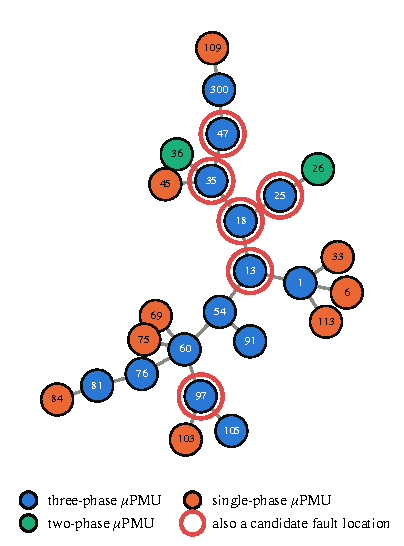
\includegraphics[width=0.42\textwidth]{fig1_1_feeder_graph.pdf}
\caption{The IEEE 123-bus feeder and the measured-only graph used in this thesis.}
\label{fig:feeder}
\end{figure}

\section{Problem Definition}

\subsection{Fault Localization Task}

Let $N=25$ be the number of instrumented buses. A window of measurements contains $S=20$ consecutive samples taken 1 ms apart. Each sample of each sensor has $F=6$ channels: the \ac{RMS} voltage magnitudes of the three phases, $V_{v,s,1}$, $V_{v,s,2}$ and $V_{v,s,3}$, and three availability-mask channels $m_{v,1}$, $m_{v,2}$ and $m_{v,3}$. A mask channel equals one when the corresponding phase is measured and zero when the phase is not installed or the sensor is lost. One window is therefore a tensor $X\in\mathbb{R}^{N\times S\times F}$. The measured-only graph $\mathcal{G}=(\mathcal{V},\mathcal{E})$ has the $N$ sensor buses as nodes and 24 edges that form a tree.

The task is to learn a model
\begin{equation}
f_{\theta}:\ \mathbb{R}^{N\times S\times F}\rightarrow\{0,1,\dots,25\},\qquad \hat{y}=f_{\theta}(X),
\label{eq:task}
\end{equation}
where class 0 means that no fault is present and classes 1 to 25 denote the faulted bus. The model returns one prediction per window. The primary performance measure is the macro-averaged F1 score over the 26 classes, called macro-F1 in the remainder of the thesis. Chapter~\ref{chap:proposed} defines it precisely.

\subsection{Sensor Loss at Inference}

A deployed \ac{UPMU} can stop reporting because of a communication failure or a hardware fault. The thesis models this event by selecting a set $\mathcal{D}$ of $k$ sensors and setting all channels of the selected sensors to zero. The model parameters stay fixed, so the evaluation measures how the model behaves when the input differs from the input seen in training. The thesis varies $k\in\{0,1,2,5,10\}$, which removes between 0 and 40\% of the sensors. The central question is how much the macro-F1 score falls as $k$ grows and how the loss can be reduced.

\subsection{Measurement Noise and Unseen Fault Conditions}

Real measurements carry noise. The thesis adds Gaussian noise to the voltage channels of the sensors that still report. The noise level is given in per-unit voltage, so that it has the same physical meaning for every phase. Together with the sensor loss of the previous subsection, the two perturbations of the input are
\begin{align}
\tilde{X}_{v,s,c} &=
\begin{cases}
0, & v\in\mathcal{D},\\
X_{v,s,c}, & v\notin\mathcal{D},
\end{cases}
\qquad |\mathcal{D}|=k, \label{eq:dropout}\\
\hat{V}_{v,s,p} &= V_{v,s,p}+\varepsilon_{v,s,p},
\qquad \varepsilon_{v,s,p}\sim\mathcal{N}(0,\sigma^{2}),\quad v\notin\mathcal{D},\ m_{v,p}=1. \label{eq:noise}
\end{align}
The training data cover only three fault resistances. A model that has learned from data alone has no knowledge of the electrical laws that connect a fault to the voltages at the sensors, so it has no principled way to handle conditions that the data do not cover. This observation motivates the second part of the thesis, which asks whether a fixed physical model of the feeder can supply information that the learned model lacks.

\section{Conditions Beyond the Training Distribution}

A monitoring system leaves the controlled conditions of a laboratory benchmark as soon as it is deployed. A \ac{UPMU} depends on a communication link and on periodic maintenance, so on a feeder with 25 units the loss of a few of them is an ordinary operating event. Field measurements are never exact, and the synchrophasor standard IEEE C37.118 limits the total vector error to one percent. A fault resistance in the field can take any value, whereas a training corpus contains a finite set of values.

The measurements reported in Chapter~\ref{chap:results} show that a purely data-driven \ac{STGNN} is sensitive to the first two conditions. The best baseline, RGSAGE-Max, reaches a macro-F1 of 0.846 when all sensors report. When 10 of the 25 sensors are removed, its macro-F1 falls to 0.048, so it keeps only 5.7\% of its clean score. When the single sensor nearest to the fault is removed, the score falls to 0.448, compared with 0.736 when one randomly chosen sensor is removed. Noise with a standard deviation of 0.01 p.u., which equals the one percent limit of the standard, lowers the score from 0.846 to 0.345.

\section{Research Gap}

Three gaps follow from the closest prior work, which Chapter~\ref{chap:survey} reviews.

\begin{enumerate}
\item \textbf{No study of sensor loss at inference for \ac{STGNN} localization.} \citet{karabulut2026} evaluate their models with a complete and fixed sensor set. \citet{chen2020} harden a static, single-snapshot classifier against measurement noise and data loss, and \citet{zhang2025} reconstruct missing measurements with graph imputation, but neither studies a spatio-temporal model whose sensors fail after deployment.
\item \textbf{No comparison of mitigation strategies under inference-time failure.} The imputation method of \citet{zhang2025} assumes that the set of unmeasured buses is fixed and known when the imputer and the classifier are built, which an inference-time failure does not provide. It is open whether a training-time method, an architectural change or an imputation step recovers the lost accuracy best.
\item \textbf{No test of fixed physical knowledge in a learned localizer under noise and loss.} Physics-based methods need dense measurements, and learned methods ignore the electrical laws. Whether a fixed physical model of the feeder complements a learned model under noise, sensor loss and unseen conditions has not been measured on this task. The thesis screens three ways to add first-order physical knowledge through the graph, a prior and the loss. None of them improved on the learned model, which shows that the form in which physics enters matters.
\end{enumerate}

\section{Research Questions}
\label{sec:rq}

The thesis addresses five research questions.

\begin{enumerate}
\item[RQ1.] How much does the accuracy of \ac{STGNN} localization fall when \acp{UPMU} are lost at inference, and does clean accuracy predict robustness?
\item[RQ2.] Can a change in training, an architectural gate or an imputation step recover the lost accuracy, and at what cost?
\item[RQ3.] Do the conclusions hold under harder loss patterns, under measurement noise and on unseen fault scenarios?
\item[RQ4.] How much information about the fault location do 25 magnitude-only sensors carry when it is measured with a physical model of the feeder, and does this information complement a learned model?
\item[RQ5.] Can the physical model be fused with the learned model without adding capacity or leaking labels, and under which perturbations does the fusion help?
\end{enumerate}

\section{Contributions}

The thesis makes the following contributions. The results on dropout-aware training have been accepted for publication \citep{sangameswar2026}.

\begin{enumerate}
\item \textbf{A multi-seed benchmark.} Five models of the \ac{STGNN} family are trained on a regenerated corpus of 1.65 million windows at three seeds each. The thesis reports its own numbers and does not claim to reproduce those of the base paper. All models share splits and mask seeds, and the comparisons use paired tests over training seeds with multiple-comparison correction.
\item \textbf{Dropout-aware training.} Randomly masking sensors during training raises the retention of RGSAGE-Max at 40\% sensor loss from 5.7\% to 80.3\%, with no added parameters or inference latency, and it outperforms neighbor-mean and learned imputation. The availability-gated \ac{SDR-STGNN} matches the method but does not exceed it, and the thesis reports this negative result as it is.
\item \textbf{A broader robustness analysis.} The conclusions are tested under worst-case, persistent and clustered sensor loss, under measurement noise, with a wider training grid and on a scenario-held-out split. The remedy does not help against measurement noise, which identifies the limit of a mask-based remedy.
\item \textbf{A physical operator and its use.} A table of fault signatures solved with a circuit simulator defines a fixed, parameter-free residual. The thesis uses it to measure identifiability, as a training-free localizer called \ac{PSM}, for imputation of lost sensors and for inference-time fusion.
\item \textbf{A physics-consistent model.} The \ac{PC-STGNN} adds one learned scalar to the dropout-aware backbone and reduces exactly to it when the physical terms are switched off. On the validation split, it scores higher than a noise-augmented reference in every seed at every combination of noise and sensor loss that was tested.
\end{enumerate}

\section{Scope and Assumptions}
\label{sec:scope}

The conclusions of the thesis hold within the following limits.

\begin{itemize}
\item All data come from simulation of one feeder, the IEEE 123-bus feeder in its default topology. The thesis does not claim that the results transfer to other feeders or to field data.
\item The measurements are \ac{RMS} voltage magnitudes from a quasi-static solver, so they contain no electromagnetic transients, no traveling waves and no sub-cycle content. Real-time localization on field streams is not demonstrated.
\item The placement of the 25 sensors is taken unchanged from the base paper. The corpus is noise-free, and noise appears only as a controlled perturbation.
\item Each simulated event uses a single global load multiplier and one of three fault resistances. The 70/15/15 partition is made over events, so each fault scenario appears in all three splits with different load levels.
\item The signature table is built with the same simulator that generated the corpus, so a comparison on clean data favors the physical operator, and the thesis draws its conclusions from the perturbed conditions. The operator is called physics-consistent and not physics-informed, and the thesis makes no claim about Kirchhoff residuals or power-flow constraints.
\item Every result with several seeds uses three training seeds. This number limits the statistical power, and the thesis states which orderings are consistent observations and which are significant.
\end{itemize}

\section{Methodology and Organization}

All experiments follow four rules. First, only one factor changes between two compared models. Second, all models use the same frozen data, the same splits and the same sensor-loss masks. Third, hyperparameters and checkpoints are selected on the validation split only, and the test split serves only for reporting. Fourth, inexpensive checks that need no training are run before an expensive training run. Chapter~\ref{chap:survey} reviews the literature, Chapter~\ref{chap:proposed} describes the methods, Chapter~\ref{chap:results} presents the results, and Chapter~\ref{chap:conclusion} summarizes the findings, states the limitations and outlines future work.

%------------------------------------------------------------------------------------------------%
% The chapters below are written one at a time. Only the headings exist so far.
\chapter{Literature Survey}
\label{chap:survey}

This chapter reviews the work on which the thesis builds, from methods that rely on circuit physics, through learning methods that ignore the network structure, to graph-based and spatio-temporal models. It then examines how the literature treats missing and noisy measurements and how physical knowledge has been combined with graph learning, and it ends with what the literature leaves open.

\section{Overview of Approaches}
\label{sec:overview}

The approaches to fault localization in distribution grids fall into four families. Circuit-based methods compute the position of the fault from impedances or from wave propagation. Learning methods with hand-crafted features map signatures of the measurements to a fault location. Graph-based learning methods represent the feeder as a graph, and spatio-temporal variants add a temporal encoder. Physics-aware learning methods combine a learned model with knowledge of the electrical laws.

\section{Circuit-Based Fault Location}

Impedance-based methods are the longest established family. They measure voltage and current at one point of the feeder, usually the substation, compute the apparent impedance and convert it into a distance. On a branching feeder, a single measured impedance corresponds to several candidate positions. A generalized one-end formulation resolves this ambiguity \citep{krishnathevar2012}. The accuracy depends on accurate line parameters, and the fault resistance disturbs the estimate.

Traveling-wave methods follow a different principle. A fault launches a wavefront that travels along the line, and the arrival times at the measurement points identify the fault position. \citet{liu2023} locate faults on multi-branch distribution networks by sharpening the arrival instants of the wavefront with an improved ensemble empirical mode decomposition and the Teager energy operator. They are largely independent of the fault resistance, but they need devices that sample at a very high rate at many points.

Both families assume a measurement coverage that is dense enough to observe the impedances or the wavefronts of interest, and neither represents which buses are electrically adjacent. Neither assumption holds on a feeder that carries a few \acp{UPMU}.

\section{Feature-Based Learning Methods}

Learning methods avoid the need for an exact circuit model. They learn the mapping from the measured signature of a fault to its location from simulated or recorded events. \citet{livani2013} identify the faulted line of the IEEE 123-bus feeder with a \ac{SVM} that uses post-fault \ac{RMS} voltages and fault-current-indicator signals. The flat feature vector of this model cannot use the adjacency of buses, which motivates the graph-based methods of the next section.

\section{Graph Neural Networks for Fault Location}

\subsection{Message Passing on the Feeder Graph}

A \ac{GNN} computes a representation for each node of a graph by repeated exchange of information with the neighbors of the node. A general layer has the form
\begin{equation}
h_v^{(l+1)}=\phi^{(l)}\Big(h_v^{(l)},\ \mathrm{AGG}\big(\{h_u^{(l)}:u\in\mathcal{N}(v)\}\big)\Big),
\label{eq:mp}
\end{equation}
where $h_v^{(l)}$ is the representation of node $v$ after $l$ layers, $\mathcal{N}(v)$ is the set of neighbors of $v$, $\mathrm{AGG}$ is a permutation-invariant aggregation, and $\phi^{(l)}$ is a learnable update. The choice of $\mathrm{AGG}$ defines the architecture. A \ac{GCN} \citep{kipf2016} aggregates with a normalized sum, GraphSAGE \citep{hamilton2017} concatenates the node with a mean or max of its neighbors, and GATv2 \citep{brody2022} weights the neighbors with learned attention coefficients. After $L$ layers, a node holds information from nodes at most $L$ hops away. This property is what lets a \ac{GNN} infer a fault at a bus that carries no sensor, because the evidence from the nearest sensors reaches the node through the graph. \citet{liao2021} survey the use of \acp{GNN} in power systems.

\subsection{Graph-Based Fault Location Models}

\citet{chen2020} apply a spectral graph convolutional network with Chebyshev filters to the IEEE 123- and 37-bus feeders. They add a data augmentation against measurement noise and data loss, which is the closest precedent for the training-time mitigation studied in this thesis. Their model, however, classifies a single snapshot over the graph of the full grid. \citet{fan2024} pair a variational graph autoencoder with GraphSAGE to recover latent node information under noise, and they also classify a single snapshot.

A temporal encoder supplies the time axis. \citet{nguyen2022} combine a one-dimensional convolutional network with a graph convolutional network, and \citet{ngo2025} combine one with graph attention, both for fault detection and identification in distribution systems.

\citet{li2021ppgn} propose a physics-preserved graph network for fault location with limited observation and limited labels, evaluated on the IEEE 123- and 37-node feeders with varying loads and topology. In this model the observability is sparse but fixed, and the set of available sensors is not varied after training.

\section{Spatio-Temporal Graph Models and the Measured-Only Graph}

\citet{karabulut2026} give the most complete treatment of spatio-temporal learning for fault location under partial observability, and their framework is the starting point of this thesis. Their pipeline combines a recurrent network that encodes the voltage history of each sensor with a spatial \ac{GNN}. They benchmark GraphSAGE and GATv2 encoders, called RGSAGE and RGATv2, against a graph convolutional encoder, called RGCN, and against a recurrent baseline, on the IEEE 123-bus feeder. The letter R in these names refers to the recurrent front end. They also propose a measured-only graph, whose nodes are only the instrumented buses, in place of the full topology of the grid. They report that all spatio-temporal variants outperform the purely recurrent baseline by up to 11 percentage points of F1, that the variants are more stable across runs, and that the measured-only graph reduces the training time six-fold and improves the F1 score by up to 11 points compared with the full topology.

A companion study by the same authors \citep{karabulut2025} benchmarks the same family of encoders for fault detection and examines how well they generalize to grid configurations that differ from those used in training. They report that RGATv2 loses about 12\% of its F1 score across topology settings, other variants of the family lose up to about 25\%, and purely recurrent models lose up to about 60\%. It varies the topology but not the availability of the sensors.

The same template of a temporal encoder followed by a graph network appears in other domains. \citet{sachin2025} cast spatio-temporal forecasting as an adaptive encoder-decoder graph network, \citet{jayapal2025} classify cancer metastasis on a graph of segmented lymph-node regions, and \citet{asiri2025} identify illicit Bitcoin transactions with a graph convolutional network, all with gains over models that do not use the graph.

\section{Missing and Noisy Measurements}

\subsection{Imputation and Reconstruction}

The most developed treatment of missing data in fault location is the work of \citet{zhang2025}. A training-free graph Dirichlet imputation reconstructs the missing bus measurements by minimizing the Dirichlet energy of the graph, and a graph convolutional network trained with contrastive learning keeps the fault signatures separable under the resulting scarcity. The method assumes that the set of unmeasured buses is a fixed property of the network that is known when the imputer and the classifier are built. A sensor that fails after deployment does not satisfy this assumption.

The idea is not specific to fault location. \citet{rossi2021} propose Feature Propagation, which minimizes the Dirichlet energy to fill missing node features and loses only about 4\% relative accuracy in node classification when 99\% of the features are missing. The features there are missing before training, so the relation to the loss of a whole sensor at inference time is indirect.

\subsection{Robustness to Sensor Failure}

Work on sensors that fail at inference time is rare outside power systems. \citet{kirthan2026} combine diffusion graph convolutions and dilated temporal convolutions with Monte Carlo dropout to separate aleatoric from epistemic uncertainty in traffic flow prediction, and they report that the model holds up better than three spatio-temporal baselines when sensors drop out. In fault localization, the predicted quantity is a discrete location that is usually not instrumented, so a lost \ac{UPMU} withdraws evidence about buses other than its own.

\subsection{Masking During Training}

Randomly removing parts of a graph during training is a known regularizer. DropEdge \citep{rong2020} removes edges at random to slow down over-smoothing and over-fitting in deep graph convolutional networks. Masking measurement nodes during training is a related operation on the input features instead of the edges. The thesis does not claim the masking primitive as new. Its contribution is to frame sensor loss as a mismatch between training and deployment conditions and to measure the effect of the remedy against several alternatives.

\section{Physics-Aware Learning for Power Systems}

Physics-informed graph learning incorporates physical rules into graph learning, and \citet{peng2022} review the methods in a unified framework. \citet{nyangon2026} review hybrid physics-informed architectures for electricity systems, including \acp{PINN} and their graph-based variants, and they name training instability, computational cost and the absence of standard benchmarks as persistent challenges. \citet{okoyomon2025} compare three strategies for voltage prediction in distribution grids, in which a physical term enters the loss, the architecture or the task formulation, and they assess both standard and out-of-distribution performance. \citet{dogoulis2025} impose Kirchhoff's current law (\ac{KCL}) as a hard constraint on the output of a graph network by projection onto hyperplanes, which yields power flow predictions without violations of the law.

Most of these methods need quantities that the data of this thesis do not contain. A Kirchhoff residual needs complex voltages or currents, whereas the \acp{UPMU} of the benchmark report \ac{RMS} voltage magnitudes only, and residuals of this kind cannot be formed from magnitudes alone.

The thesis therefore uses a different form of physical knowledge. A circuit simulator solves the feeder for every candidate fault, and the resulting signatures define a fixed residual between a measurement and each hypothesis. This residual needs no complex quantities, and it contains no learned parameter. The thesis calls this knowledge physics-consistent and does not call it physics-informed in the sense of a differential-equation residual.

\section{Summary and Research Gap}

The survey leads to four observations that define the research gap of this thesis.

\begin{enumerate}
\item Spatio-temporal graph models are the most capable family for fault localization under partial observability, but the existing evaluations assume that every sensor reports at all times. No study measures how these models degrade when whole sensors fail after deployment.
\item The remedies in the literature for missing data assume a fixed pattern of missingness that is known in advance, or they address noise and data loss in static classifiers. It is not known whether a training-time method, an architectural change or an imputation step recovers the accuracy lost to an inference-time sensor failure, and at what cost.
\item The evaluations use a single missingness model or none, so it is not known whether a remedy transfers to worst-case, persistent, clustered or noisy conditions.
\item Physics-aware methods rely on complex quantities or on fixed observability. How much a fixed physical model of the feeder adds to a learned localizer that sees only magnitudes, and under which perturbations it adds it, has not been measured on this task.
\end{enumerate}

\chapter{Proposed Work}
\label{chap:proposed}

This chapter describes the methods in the order in which they build on one another: the simulated corpus (Section~\ref{sec:data}), the five baseline models (Section~\ref{sec:baselines}), the sensor-loss protocol (Section~\ref{sec:protocol}), dropout-aware training, the availability-gated model and the stress-test methods (Sections~\ref{sec:dropaware} to~\ref{sec:stress}), and the physical operator and the physics-consistent model (Sections~\ref{sec:physics} and~\ref{sec:pcstgnn}).

\section{Simulation and Dataset}
\label{sec:data}

\subsection{Feeder and Scenario Design}

The corpus is generated by simulation of the IEEE 123-bus distribution feeder, a standard radial benchmark with a nominal line-to-line voltage of 4.16 kV at 60 Hz. The simulator is OpenDSS, driven through its Python interface. The simulation runs in daily (quasi-static time-series) mode with a step of 1 ms. Each recorded sample is therefore a converged power-flow solution and not a single operating-point snapshot. The corpus describes the post-inception \ac{RMS} depression of the voltage and its spatial pattern over the feeder.

The scenarios follow the factorial design of \citet{karabulut2026}. Faults are injected at 25 candidate buses, with 11 fault types and 3 fault resistances, which gives 825 scenarios. The fault types are the three line-to-ground faults, the three line-to-line faults, the three double-line-to-ground faults and two three-phase faults, one with and one without ground. The fault resistances are 0.1, 1 and 10~$\Omega$. Each scenario is simulated 50 times, which gives 41,250 events. A run draws one global load multiplier $\eta$ from the uniform distribution on $[0.5,1.3]$ and applies it to every load of the feeder, so the 50 runs of a scenario differ only in the load level.

\subsection{Sensors and the Measured-Only Graph}

The sensors follow the placement of \citet{karabulut2026}. Twenty-five buses carry a \ac{UPMU}: buses 1, 6, 13, 18, 25, 26, 33, 35, 36, 45, 47, 54, 60, 69, 75, 76, 81, 84, 91, 97, 103, 105, 109, 113 and 300. Fourteen of them measure all three phases. The other eleven measure one or two phases, so 55 of the 75 phase channels are instrumented. A channel that is not instrumented carries a voltage of zero and an availability mask of zero. Only six of the 25 candidate fault buses (13, 18, 25, 35, 47 and 97) coincide with an instrumented bus.

The measured-only graph has the 25 instrumented buses as nodes. Its edges follow a breadth-first spanning tree of the feeder that is rooted at the substation, bus 150. Each unit is connected to the nearest instrumented unit upstream of it on this tree. One exception keeps the graph connected: a single- or two-phase unit whose nearest upstream unit is also single- or two-phase is not connected to that unit. Two units, at buses 33 and 113, are in this case, and a fallback connects each of them along the shortest feeder path to the unit at bus 1. The result is a connected tree with 24 edges. Figure~\ref{fig:feeder} in Chapter~\ref{chap:intro} shows the graph.

\subsection{Windows, Labels, Splits and Normalization}

An event is recorded for 60 ms. The fault is injected at step 40, so the record has 40 steps before the fault and 20 steps with the fault. Windows of 20 samples are cut with a stride of 1 ms, and the first 40 windows are kept, with start steps from 0 to 39. Windows 0 to 19 end before the fault and have the label no fault. Windows 20 to 39 end after the fault starts and carry the label of the faulted bus. Window $w$ therefore contains $w-20$ samples after fault inception. Every event contributes 20 windows of each kind, so exactly half of the 1.65 million windows belong to the no-fault class and the 25 fault classes are equally frequent.

The partition into training, validation and test data is made at the event level, stratified by fault bus, with the proportions 70, 15 and 15 percent. All 40 windows of an event stay in one split, and the measured overlap of events between any two splits is zero. The training split holds 28,875 events (1,155,000 windows), the validation split 6,200 events (248,000 windows) and the test split 6,175 events (247,000 windows), and exactly half of the windows of each split are no-fault windows. Each fault scenario appears in all three splits with different load levels, so the split measures generalization to unseen load conditions of a known fault configuration. Section~\ref{sec:scenario} describes the complementary split that holds out scenarios.


The voltage channels are normalized to zero mean and unit variance per phase with statistics of the training split. The mask channels stay binary. The mask channels are static in the clean corpus: they encode which phases each unit measures and are identical in every window. This property matters for the interpretation of dropout-aware training in Chapter~\ref{chap:results}.

\subsection{Data Quality and Reference Bounds}

Several checks were run on the whole corpus and not on samples. After the second post-fault step the voltage level is constant to within $1.1\times10^{-7}$ p.u. in all 41,250 events, so the fault period is quasi-static. Two reference bounds follow from the window design. A classifier that always answers no fault reaches a macro-F1 of 0.0256, which serves as the trivial reference. Window 20 of every fault event carries a fault label but contains no post-fault sample, so it is physically identical to a healthy window. No model can beat chance on these windows, and they lower the best achievable macro-F1 to 0.9744. They make up 2.5\% of the test split, and the accuracy of every trained model on this subset lies between 0.0003 and 0.0418 against a chance rate of 0.0385, which shows that no label information leaks into the inputs.

\subsection{Scenario-Held-Out Split}
\label{sec:scenario}

The event-level split leaves every scenario in all three splits. To test generalization to unseen fault configurations, a second split assigns whole scenarios to one split. The assignment is made within each fault bus, so all 25 fault classes remain present in every split, and what is withheld is the combination of fault type and resistance at that bus. The split has 575 training scenarios, 125 validation scenarios and 125 test scenarios, with no overlap, and it covers 28,750, 6,250 and 6,250 events.

\section{Baseline Architectures}
\label{sec:baselines}

\subsection{Shared Template}

The five baseline models follow the framework of \citet{karabulut2026}. A temporal encoder produces one embedding per instrumented bus, an optional spatial stage exchanges information over the measured-only graph, and a shared classifier assigns class probabilities to each node. A soft vote over the nodes yields the prediction for the window. Let $x_v\in\mathbb{R}^{S\times F}$ be the input of node $v$. A single-layer \ac{GRU} with 128 hidden units, shared by all nodes, encodes it:
\begin{equation}
h_v^{(0)}=\mathrm{GRU}(x_v)\in\mathbb{R}^{128},\qquad v=1,\dots,N.
\label{eq:gru}
\end{equation}
The model that consists of this encoder and the classifier alone is the recurrent baseline, called GRU in the tables. It has no message-passing stage and is therefore not a spatio-temporal graph model.

\subsection{Spatial Encoders}

The four graph models stack $N_{\mathrm{hop}}=4$ message-passing layers with a hidden dimension of 64 and self-loops. They differ only in the aggregation operator. Let $\tilde{\mathcal{N}}(j)=\mathcal{N}(j)\cup\{j\}$ be the closed neighborhood of node $j$. RGCN propagates over the symmetrically normalized adjacency $\tilde{D}^{-1/2}\tilde{A}\tilde{D}^{-1/2}$ \citep{kipf2016}. RGSAGE concatenates the representation of a node with a mean-pooled or max-pooled aggregate of its neighbors \citep{hamilton2017}, which gives the variants RGSAGE-Mean and RGSAGE-Max. RGATv2 weights the neighbors with learned attention coefficients and uses $H=4$ heads \citep{brody2022}. The three updates are
\begin{align}
h_j^{(l+1)}&=\mathrm{ReLU}\Big(\textstyle\sum_{i\in\tilde{\mathcal{N}}(j)}\tfrac{1}{\sqrt{\tilde d_i\tilde d_j}}\,h_i^{(l)}W^{(l)}\Big), \label{eq:gcn}\\
h_j^{(l+1)}&=\mathrm{ReLU}\Big(W^{(l)}\big[h_j^{(l)}\,\Vert\,\rho\big(\{h_i^{(l)}:i\in\tilde{\mathcal{N}}(j)\}\big)\big]\Big), \label{eq:sage}\\
h_j^{(l+1)}&=\mathrm{ReLU}\Big(W_{\mathrm{o}}^{(l)}\,\Big\Vert_{c=1}^{H}\sum_{i\in\tilde{\mathcal{N}}(j)}\alpha_{ji}^{(l,c)}\,W^{(l,c)}h_i^{(l)}\Big), \label{eq:gat}
\end{align}
where $\tilde d_i$ is the degree of node $i$ including the self-loop, $\Vert$ denotes concatenation, $\rho$ is the mean or the maximum, and $\alpha_{ji}^{(l,c)}$ is the attention coefficient of head $c$. The rectifier is omitted after the last layer, whose output passes directly to the classifier. The depth of four layers is a choice of this thesis: a single layer limits the receptive field of a node to its immediate neighbors, and most fault locations lie more than one hop from any instrumented bus. The depth was selected on RGSAGE-Max alone, by the diagnostic of Chapter~\ref{chap:results}, and then applied to every architecture.

A shared classifier maps the final embedding of each node to 26 logits. It consists of batch normalization, a rectifier, dropout with a rate of 0.35 and a linear layer. At inference the class probabilities of the $N$ nodes are summed, and the class with the largest sum is the prediction for the window:
\begin{equation}
\hat{y}=\arg\max_{c\in\{0,\dots,25\}}\sum_{v=1}^{N}\mathrm{softmax}(z_v)_c .
\label{eq:softvote}
\end{equation}
Training minimizes the unweighted node-level cross-entropy, in which the label of the window supervises every node,
\begin{equation}
\mathcal{L}=\frac{1}{N}\sum_{v=1}^{N}\mathrm{CE}(z_v,y).
\label{eq:loss}
\end{equation}
Class imbalance is handled by the design of the corpus, which is balanced, and not by loss weighting.

\subsection{Training Configuration}

All models share one training configuration. The optimizer is AdamW with a learning rate of $10^{-3}$ and a weight decay of $10^{-4}$, with a linear warm-up over the first 3 epochs, constant afterwards, and the gradient norm is clipped at 1.0. Training runs for 30 epochs with batches of 32 windows,. The checkpoint with the best validation graph-level macro-F1 is kept, and no other early stopping is used. Every model is trained at three seeds, 42, 43 and 44, which control the parameter initialization, the batch order and the masking of dropout-aware training. The experiments ran on one NVIDIA T1000 with 8 GB of memory, with Python 3.12, PyTorch 2.5.1 with CUDA 12.1, PyTorch Geometric 2.8, OpenDSSDirect.py 0.9.4 and scikit-learn 1.9.

\section{Sensor-Loss Evaluation Protocol}
\label{sec:protocol}

\subsection{Missingness Model}

Robustness to sensor loss is measured entirely at inference time, with all model parameters fixed. This isolates the behavior of a deployed model from any training-time remedy. The thesis draws a set $\mathcal{D}$ of $k$ of the 25 sensors for each test window and sets all six input channels of every selected node to zero, as in Eq.~\eqref{eq:dropout}. The mask channels are zeroed together with the voltages because a zero voltage can be a valid reading after normalization, so the mask is the only definitive indicator that a node is unobserved. A unit that fails is thus encoded like a phase that was never installed. A dropped node keeps its edges and takes part in message passing. Its temporal encoder receives an all-zero sequence, and the resulting embedding propagates to its neighbors.

The study uses $k\in\{0,1,2,5,10\}$, which removes 0, 4, 8, 20 and 40\% of the sensors. For $k>0$ the selected nodes are drawn uniformly at random, independently for every window. The pseudo-random seed of a batch is derived from the level $k$, the index of the mask realization and the index of the batch, so that every architecture sees an identical sequence of dropped sensors on the same frozen test split. Each point of a degradation curve is averaged over three mask realizations. The three realizations are averaged within each training seed before any statistical test, so that mask realizations are not treated as independent samples. The score at $k=0$ of every degradation curve equals the clean score recorded for the checkpoint. An early version of the evaluator used the same mask seed in every batch, so the same subsets repeated; the seed is now derived from the batch index, and all dropout results were recomputed and not patched.

\subsection{Metrics}

The primary metric is the macro-averaged F1 score over the 26 classes. Each test window receives one prediction by the soft vote of Eq.~\eqref{eq:softvote}. The predictions of all 247,000 test windows are pooled, without aggregation over the 40 windows of an event. The per-class F1 scores are averaged without weighting:
\begin{equation}
\mathrm{F1}_{\mathrm{macro}}=\frac{1}{26}\sum_{c=0}^{25}\frac{2\,\mathrm{Pr}_c\,\mathrm{Re}_c}{\mathrm{Pr}_c+\mathrm{Re}_c},
\label{eq:f1}
\end{equation}
where $\mathrm{Pr}_c$ and $\mathrm{Re}_c$ are the precision and the recall of class $c$. The no-fault class holds half of the windows but only one twenty-sixth of the weight, and the macro average is used so that the 25 fault classes dominate the score. The node-level macro-F1 reported for the baselines treats the prediction of each node as a separate sample.

Two quantities describe the shape of a degradation curve. The retention at level $k$ is the score relative to the clean score, and the \ac{AUDC} is its normalized integral over the sweep:
\begin{align}
\mathrm{Ret}(k)&=\frac{\mathrm{F1}(k)}{\mathrm{F1}(0)}, \label{eq:ret}\\
\mathrm{AUDC}&=\frac{1}{k_{\max}-k_{\min}}\int_{k_{\min}}^{k_{\max}}\mathrm{Ret}(k)\,\mathrm{d}k\in[0,1], \label{eq:audc}
\end{align}
with $k_{\min}=0$ and $k_{\max}=10$ and trapezoidal integration over the five levels. A larger value means slower degradation. Both measures are relative to the clean score of the model itself, so a weak model can obtain a flattering value, and the thesis therefore also reports the absolute area, which is the same integral applied to the raw macro-F1, and it reads every score against the trivial reference of 0.0256 and the ceiling of 0.9744.

\subsection{Statistical Procedure}

Every comparison between variants is a mean over three training seeds, which is a small sample, so the thesis states which differences survive a test. The training seed is the paired unit, because all variants are trained from the same three seeds on the same data. The test is a paired two-sided $t$-test on the seed-wise differences with two degrees of freedom, reported with a 95\% confidence interval. Tests that answer one question form a family, and the Holm-Bonferroni correction is applied within each family. Every reported $p$-value is the adjusted value $p_{\mathrm{Holm}}$. A complementary cluster bootstrap resamples the 6,175 test events and not the windows, because the 40 windows of an event are correlated.

\section{Dropout-Aware Training}
\label{sec:dropaware}

The baselines are trained with all 25 sensors available but are evaluated with some sensors missing, so they are tested on inputs that differ from the inputs of training. Dropout-aware training removes this mismatch by applying the evaluation missingness model during training. For every mini-batch, a dropout level $k$ is drawn uniformly from $\mathcal{K}=\{0,1,2,5\}$. Then, independently for every window of the batch, $k$ nodes are drawn uniformly without replacement and all six channels of the selected nodes are set to zero. The masking generator is reseeded at the start of every epoch. Figure~\ref{fig:aware} shows the setup.


\begin{figure}[htbp]
\centering
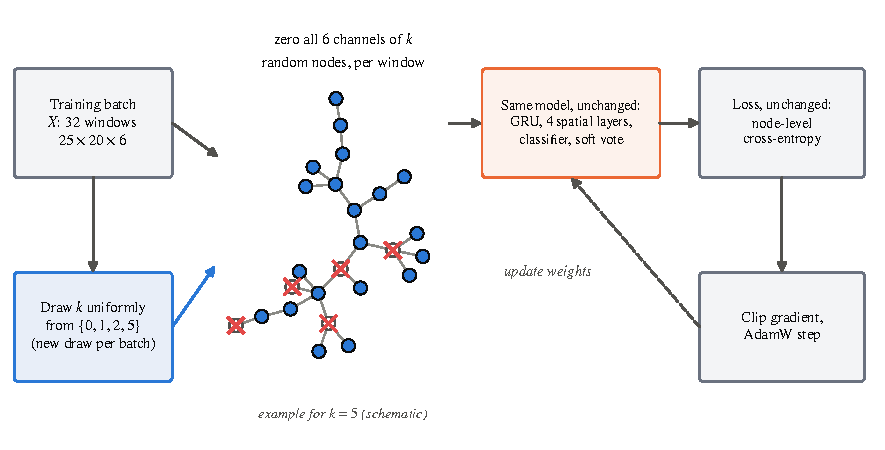
\includegraphics[width=0.55\textwidth]{fig3_0_dropout_aware.pdf}
\caption{Dropout-aware training. Only the masking of the input differs from standard training. The example graph is a schematic.}
\label{fig:aware}
\end{figure}

The augmentation touches only the input features. It changes neither the graph, the architecture, the loss nor the optimizer, so it applies without modification to every baseline and to the availability-gated model of the next section. The main configuration trains with $\mathcal{K}=\{0,1,2,5\}$ and therefore never shows the level $k=10$ of the evaluation. A variant with $\mathcal{K}=\{0,1,2,5,10\}$, called DA-wide, tests whether including the largest level helps.

\section{SDR-STGNN: Availability-Gated Aggregation}
\label{sec:sdr}

The sensor-dropout-robust spatio-temporal graph neural network, \ac{SDR-STGNN}, addresses sensor loss through the architecture and serves as an ablation against dropout-aware training. All five baselines receive the mask as input, yet none of the aggregation operators of Eqs.~\eqref{eq:gcn} to~\eqref{eq:gat} uses it, so a dropped node keeps contributing its zero-valued embedding as a non-informative message. \ac{SDR-STGNN} builds on RGSAGE-Max and makes the aggregation depend on availability. For every window, a node is available if any of its mask channels is active at any step:
\begin{equation}
a_i=\mathbf{1}\Big\{\max_{s}\max_{p\in\{1,2,3\}}m_{i,p}(s)>0\Big\}\in\{0,1\}.
\label{eq:avail}
\end{equation}
The max-pooled aggregation uses only available source nodes, and the same indicator gates the self-representation:
\begin{equation}
h_j'=\mathrm{ReLU}\Big(W\big[a_j h_j\,\Vert\,\mathrm{agg}_j\big]\Big),\qquad
\mathrm{agg}_j=\max_{\substack{i\in\tilde{\mathcal{N}}(j)\\a_i=1}}h_i,
\label{eq:gated}
\end{equation}
where $\mathrm{agg}_j=0$ if no node of the closed neighborhood of $j$ is available. Dropped nodes send no messages. The availability indicators are computed once from the input and reused in all four layers. The gate adds no parameters. When every sensor is available ($a_i=1$ for all $i$), Eq.~\eqref{eq:gated} reduces exactly to the RGSAGE-Max update, so the two models are identical at $k=0$. \ac{SDR-STGNN} is trained with the dropout-aware augmentation, so that the gates are exercised throughout training.

\section{Comparison and Stress-Test Methods}
\label{sec:stress}

The thesis tests dropout-aware training against alternative remedies and against harder conditions on the same corpus, the same splits and the same frozen checkpoints. The methods that need a physical model are described in Section~\ref{sec:physics}.


\subsection{Imputation Before Inference}

A natural alternative to training with missing data is to reconstruct the dropped sensors before inference and to present the result to a standard-trained model. The neighbor-mean imputer fills the three voltage channels of each dropped node with the per-time-step mean of its available one-hop neighbors in the undirected measured-only graph. If the whole neighborhood is dropped, the fill is zero. The mask of the imputed node is set to one, which is the most favorable setting for imputation because the model is told that the value is observed. The dropped nodes are selected exactly as in the zeroing sweep, so only the fill differs. The imputer is the training-free analogue of the graph imputation of \citet{zhang2025}.

The learned imputer is a masked autoencoder on the measured-only graph. A per-node encoder maps the flattened window and an availability flag to a vector of dimension 128 and concatenates a learned embedding of the node identity. Four residual layers with mean aggregation over the closed neighborhood follow, and a decoder returns the normalized voltages of the 20 time steps. It is trained on the training split to reconstruct the voltages of $k$ randomly dropped nodes, with $k$ drawn uniformly from 1 to 10, using AdamW at a constant learning rate of $10^{-3}$, a batch size of 64 and 60,000 steps. The checkpoint with the lowest validation reconstruction error is kept. One imputer is trained per seed and is paired with the standard-trained RGSAGE-Max of the same seed. The number of steps was decided by a rule fixed before the evaluation: an initial run of 20,000 steps was still improving by more than 2\% between steps 15,000 and 20,000, so it was repeated with 60,000 steps. Joint training of imputer and classifier is not examined.

\subsection{Harder Loss Patterns}

\textbf{Targeted loss} drops the $k$ sensors nearest to the fault. Proximity is the hop distance on the full 123-bus topology and not on the measured-only graph, because most fault buses are not nodes of the measured-only graph. The no-fault windows have no fault bus and fall back to random selection. The reported score is therefore a conservative bound on the true worst case.

\textbf{Persistent loss} draws the dropped set once per event and holds it for all 40 windows of the event, as a real failure would behave. The set is a pure function of the event, the level $k$ and the mask realization, so it is the same for every model and batch size.

\textbf{Clustered loss} drops a connected block of the measured-only graph. The block is grown from a uniformly drawn root by repeatedly adding a uniformly drawn neighbor of the current block. It models sensors that share a communication path or a feeder segment.

\subsection{Measurement Noise}

Zero-mean Gaussian noise is added to the voltage channels at inference. The standard deviation is specified in per-unit voltage and applied in normalized space as the physical value divided by the training standard deviation of the phase. The noise levels are 0.0005, 0.002 and 0.01 p.u. The largest level equals the one percent limit of the synchrophasor standard. Noise is added only where the mask is one, so unmeasured phases and dropped nodes receive none, and the mask channels are never perturbed. Noise and sensor loss are applied together on a grid of the noise level and the number $k$ of dropped sensors, on the frozen checkpoints and with the same masks as the dropout sweep.

\subsection{Classical Baselines}

To measure how much of the accuracy needs a graph model at all, a logistic regression and a random forest with 100 trees are trained on summary features. Each window is reduced, for every sensor and phase, to the minimum, mean, maximum and standard deviation over the 20 samples, and these are concatenated with the three mask values of the node. This gives 25 nodes with 15 values each, or 375 features per window. The features are standardized, and the models are trained on a subsample of 93,696 training windows with the same splits and dropout masks as the neural models.

\section{The Physical Operator}
\label{sec:physics}

\subsection{Signature Table}

The physical operator is a table of fault signatures computed with the same circuit simulator that generated the corpus. For every candidate location $f$, fault type $\tau$, fault resistance $R_{\mathrm{F}}$ and load multiplier $\eta$, one power-flow solution gives the settled post-fault voltage magnitude of each phase at each of the 25 sensors. The table is written $\mathcal{S}[f,\tau,R_{\mathrm{F}},\eta,i,p]$ in per-unit voltage. A second table $\mathcal{S}_0[\eta,i,p]$ holds the voltages of the healthy feeder at each load level, which gives the no-fault class a signature. The axes are the 25 candidate fault buses, the 11 fault types of the corpus, 18 resistances on a logarithmic grid from 0.05 to 30~$\Omega$ that contains the training values 0.1, 1 and 10~$\Omega$, and 17 load multipliers from 0.5 to 1.3 in steps of 0.05, at 75 sensor channels of which 55 are instrumented. The table holds 84,150 fault solutions and 17 healthy solutions, or 3,366 hypotheses per class.


The table is built along the path of the corpus. The feeder is compiled again for every solution, because the circuit simulator carries regulator tap positions from one solution to the next on a standing circuit, which was found to shift the signatures. The loads are set to $\eta$ times the frozen pre-fault level of the corpus, which is 0.99953, and three solver steps are taken after fault injection so that the signature is the settled level. All 84,167 solutions converged. The resistance grid contains the three corpus resistances exactly, because a grid that left them off-grid let a nearby wrong resistance trade against a compensating load shift and corrupted the recovery of the load.

A comparison on clean data tests the fidelity of the operator and cannot show that the physical model beats the learned model, as noted in Section~\ref{sec:scope}. The thesis therefore uses the operator under perturbations that the generator does not produce, namely sensor loss and measurement noise.

\subsection{Observation and Residual}

The residual compares a window with the signature of every hypothesis. The observation is the last time step of the window, converted back to per-unit voltage with the training statistics of the loader,
\begin{equation}
s_{ip}=x_{i,S,p}\,\mathrm{std}_p+\mathrm{mean}_p,\qquad \mathcal{A}=\{(i,p):m_{ip}=1\}.
\label{eq:obs}
\end{equation}
The last step is the post-fault level whenever the window contains at least one post-fault sample, because the fault period is quasi-static. The observation uses no window index, no label and no event metadata. The set $\mathcal{A}$ contains the channels that are instrumented and not dropped, so dropped sensors are handled by construction: they simply do not enter the sum.

For each class the nuisance parameters are profiled out. The type, the resistance and the load are not known, so the operator keeps the best-fitting hypothesis,
\begin{align}
r_f(\mathcal{A})&=\min_{\tau,R_{\mathrm{F}},\eta}\sum_{(i,p)\in\mathcal{A}}\frac{\big(s_{ip}-\mathcal{S}[f,\tau,R_{\mathrm{F}},\eta,i,p]\big)^2}{\sigma_\varepsilon^2+\sigma_0^2},\qquad f=1,\dots,25, \label{eq:rf}\\
r_0(\mathcal{A})&=\min_{\eta}\sum_{(i,p)\in\mathcal{A}}\frac{\big(s_{ip}-\mathcal{S}_0[\eta,i,p]\big)^2}{\sigma_\varepsilon^2+\sigma_0^2}. \label{eq:r0}
\end{align}
Here $\sigma_\varepsilon$ is a fixed floor and $\sigma_0$ is the level of the noise injected into the measurement, which is zero on the clean corpus and is set to the injected level under noise. The floor $\sigma_\varepsilon$ is a single constant, chosen on the training split only so that the median squared residual per channel at the true class equals one. Its value is $7.2555\times10^{-4}$ p.u.

The raw residuals of wrong locations are very large, of order $10^5$ to $10^6$ with this floor, whereas the residual of the true location is of the order of the number of channels. The operator therefore shifts and halves them:
\begin{equation}
\rho_f=\tfrac{1}{2}\big(r_f-\min_{g}r_g\big)\ \ge 0 .
\label{eq:rho}
\end{equation}
The quantity $\rho_f$ is in units of a Gaussian log-likelihood, so a difference of one is one nat of evidence. It is zero for exactly one class, and it does not depend on the number of available channels, which makes it comparable across dropout levels. The physics prior over the 26 classes is $P_{\mathrm{phys}}=\mathrm{softmax}(-\rho)$. Physics signature matching (\ac{PSM}) is the training-free localizer that returns the class with the smallest residual, $\hat{y}=\arg\min_f\rho_f$. The margin $\rho_{(2)}-\rho_{(1)}$ between the best and the second-best class measures how decisive the evidence is.

The residual is a function of the inputs and the fixed table, so it carries no gradient with respect to any learnable weight.

\subsection{Identifiability}

The table also measures how much the sensors can reveal in principle. For two locations $f_1$ and $f_2$, the separability is the closest approach of their two signature manifolds on the available channels,
\begin{equation}
D(f_1,f_2;\mathcal{A})=\min_{(\tau_1,R_1,\eta_1),(\tau_2,R_2,\eta_2)}\sum_{(i,p)\in\mathcal{A}}\frac{\big(\mathcal{S}_{f_1}-\mathcal{S}_{f_2}\big)^2}{2(\sigma_\varepsilon^2+\sigma_0^2)} ,
\label{eq:sep}
\end{equation}
which is in the same units as $\rho$. It is the residual that a perfect observation of $f_1$ would assign to $f_2$, and a value below one means that the two locations are indistinguishable at the floor of the operator. The thesis averages $D$ over random sensor subsets for each $k$ and reports the fraction of location pairs with $D<1$ per resistance. It is compared with an empirical measure that uses no table: the nearest-neighbor confusion between training events at different locations, computed on the raw observations.

\subsection{Physics-Based Imputation and Inference-Time Fusion}

Two further uses of the operator need no training. In physics-based imputation, each dropped node is filled with the signature of the best hypothesis of \ac{PSM}, profiled on the available channels only. The fill is normalized with the training statistics, repeated over the 20 time steps, and presented with a mask of one to the standard-trained RGSAGE-Max, so the comparison with the neighbor-mean fill isolates the fill.

In inference-time fusion, the residual is combined with the logits of an existing trained model without retraining. The logits of every node are reduced by a multiple of the residual,
\begin{equation}
z'_{n,f}=z_{n,f}-\beta\,\rho_f(\mathcal{A}),
\label{eq:fusion}
\end{equation}
where the same $\rho_f$ is used for every node $n$ and $\beta\ge0$ is chosen on validation data from the grid $\{0,0.1,0.25,0.5,1,2,4,8,16\}$. The result is then soft-voted as before.

\section{PC-STGNN: Physics-Consistent Fusion in the Network}
\label{sec:pcstgnn}

\subsection{Architecture}

The physics-consistent spatio-temporal graph neural network, \ac{PC-STGNN}, keeps the dropout-aware RGSAGE-Max backbone unchanged and fuses the residual into the logits of every node before the soft vote, as in Eq.~\eqref{eq:fusion}, with $\beta$ now a learned scalar initialized to zero. Every node distribution is thus multiplied by the same physics prior, $\exp(-\beta\rho_f)$, before the votes are summed, which is a product of experts per node. The physical path adds exactly one learned parameter, so the model has 95,259 parameters against 95,258 for the backbone, and the signature tables and the floor are fixed buffers that receive no gradient. Figure~\ref{fig:pcstgnn} shows the architecture.

\begin{figure}[htbp]
\centering
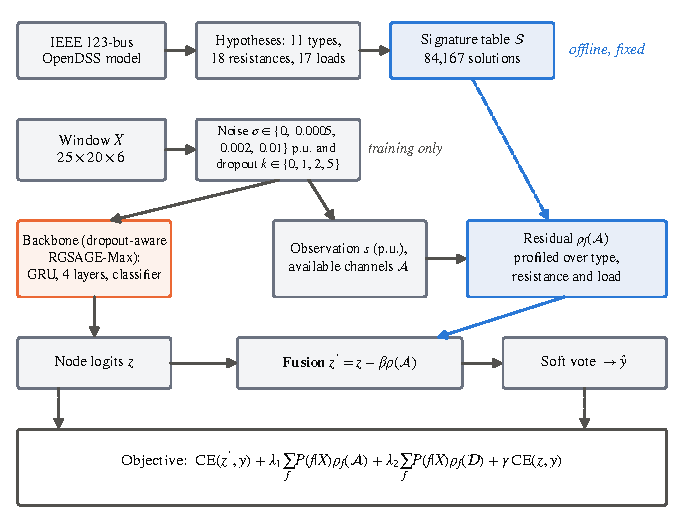
\includegraphics[width=0.72\textwidth]{fig3_2_pcstgnn.pdf}
\caption{Architecture of \acs{PC-STGNN}.}
\label{fig:pcstgnn}
\end{figure}

\subsection{Training Objective}

Let $z$ be the node logits of the backbone and $z'$ the fused logits. The objective has three terms besides the main cross-entropy:
\begin{equation}
\mathcal{L}_{\mathrm{PC}}=\mathrm{CE}(z',y)+\lambda_1\sum_{f}P(f|X)\,\rho_f(\mathcal{A})+\lambda_2\sum_{f}P(f|X)\,\rho_f(\mathcal{D})+\gamma\,\mathrm{CE}(z,y).
\label{eq:pcloss}
\end{equation}
Here $P(f|X)$ is the normalized soft-vote distribution of the model. The second term is the expected residual on the available sensors. The third is a leave-$k$-out consistency term: the hypothesis that was profiled on the available sensors is scored on the sensors $\mathcal{D}$ that were dropped in training, whose true values are known at training time only. The profiling never sees $\mathcal{D}$, so the term is a consistency check and not a reconstruction loss. The two physical terms act on the network through $P(f|X)$ and not through the residual. The last term is a cross-entropy on the logits of the network alone, before fusion. Its weight is fixed at $\gamma=1$ and is not tuned. Windows with no post-fault sample, window 20 of every fault event, are excluded from the two physical terms, because the physics correctly prefers the no-fault class there. This is the only use of the window index, and it applies in training only.

\subsection{Noise Augmentation and Collapse Guard}

On the noise-free corpus the residual at the true class is exactly zero, so the easiest solution for the fusion is to trust the physics completely and to let the network contribute nothing. Training under noise gives the physical term a finite and informative dynamic range. PC-STGNN is therefore trained with measurement noise on top of dropout-aware training. For every window, a noise level is drawn from $\{0,0.0005,0.002,0.01\}$ p.u., with zero among the choices so that clean inputs remain in the data. Noise is added before the dropout is applied, the dropout levels are $\mathcal{K}=\{0,1,2,5\}$ as before, and $\sigma_0$ in the residual is set to the level injected into each window.

The noise is included so that the model is robust to measurement noise, and the auxiliary term of Eq.~\eqref{eq:pcloss} is included to keep the network branch from collapsing. A collapse guard monitors the network branch alone on the validation split at $k=0$ without noise. An arm collapsed if the network-only macro-F1 is at most 0.10 or if more than 95\% of its predictions are no fault. A collapsed arm is not eligible for selection, and a run that is collapsed at the end of epoch 3 is stopped.

\subsection{Selection Rules, Reference Model and Verification}

The weights $\lambda_1$ and $\lambda_2$ are chosen on the validation split by the macro-F1 averaged over $k\in\{0,1,2,5,10\}$ among the arms that pass the collapse guard, with one seed and 15 epochs per arm. The grid is $\lambda_1\in\{0,0.01,0.0333,0.1\}$ with $\lambda_2=0$, followed by one arm with $\lambda_2=0.1$ at the best $\lambda_1$. Tuning runs never evaluate the test split.

The reference for every comparison is a model with the same recipe and no physics: the dropout-aware RGSAGE-Max with the same noise augmentation, called the noise-augmented reference model. Comparing PC-STGNN with a model trained without noise would confound noise augmentation with physics, so both models are trained with the same augmentation, for 30 epochs and at three seeds. Both are evaluated on the validation split on the grid of the noise levels $\{0,0.0005,0.002,0.01\}$ p.u. and the sensor-loss levels $k\in\{0,1,2,5,10\}$, with three mask realizations.

Two checks guard the implementation before any training result is trusted. In the null test, a PC-STGNN with $\lambda_1=\lambda_2=\beta=0$ is trained from seed 42 and must reproduce the per-epoch loss and validation score of the dropout-aware backbone exactly. A second null test shows that $\gamma=0$ reproduces the old objective and its gradients exactly on a fixed batch. In the gradient audit, finite differences on three deliberately chosen batches confirm that both physical terms send a gradient to the network weights and that the signature table receives none. The batches contain a window 20, a high dropout level and a batch with no dropped sensors.



\chapter{Results and Inferences}
\label{chap:results}

This chapter reports the measurements and what they imply. Unless stated otherwise, scores are the soft-voted macro-F1 on the frozen test split, given as mean $\pm$ standard deviation over the training seeds 42, 43 and 44, and every dropout result averages three mask realizations within each seed. Results of the physical operator that use the validation split are labeled as such, because the test split is not used for any decision or tuning.

\section{Baseline Accuracy Under Full Observability}

Table~\ref{tab:baseline} gives the five baselines with all sensors reporting. The four spatio-temporal graph models clearly outperform the recurrent baseline, which shows that message passing matters when only six of the 25 fault locations carry a sensor. RGSAGE-Max is the most accurate model, with a macro-F1 of $0.846\pm0.007$. The graph-level score exceeds the node-level score for every model, so the soft vote improves on the prediction of any single node. Accuracy falls as the fault resistance rises: RGSAGE-Max drops from 0.949 at 0.1~$\Omega$ to 0.676 at 10~$\Omega$, which agrees with the weak voltage signature of high-impedance faults. Fault detection is saturated, since every model reaches a no-fault recall of at least 0.9999 and a precision of at least 0.972, so the difficulty lies in localization. RGATv2 is the weakest graph model and the least stable across seeds. At the adopted depth of four layers, its variance suggests a training instability that was not addressed.

\begin{table}[htbp]
\caption{Baseline macro-F1 under full observability, mean $\pm$ standard deviation over three seeds. The best value per column is in bold.}
\label{tab:baseline}
\small
\centering
\begin{tabular}{@{}lcccccc@{}}
\toprule
 & \multicolumn{2}{c}{Macro-F1} & \multicolumn{3}{c}{Graph-level by resistance} \\
\cmidrule(lr){2-3}\cmidrule(lr){4-6}
Model & Graph & Node & 0.1~$\Omega$ & 1~$\Omega$ & 10~$\Omega$ \\
\midrule
RGSAGE-Max & \textbf{0.846}$\pm$0.007 & \textbf{0.718}$\pm$0.008 & \textbf{0.949} & \textbf{0.893} & \textbf{0.676} \\
RGSAGE-Mean & 0.786$\pm$0.023 & 0.660$\pm$0.025 & 0.906 & 0.843 & 0.587 \\
RGCN & 0.712$\pm$0.017 & 0.601$\pm$0.019 & 0.874 & 0.792 & 0.428 \\
RGATv2 & 0.522$\pm$0.087 & 0.460$\pm$0.080 & 0.630 & 0.574 & 0.312 \\
GRU & 0.286$\pm$0.009 & 0.150$\pm$0.003 & 0.410 & 0.292 & 0.105 \\
\bottomrule
\end{tabular}
\end{table}

The choice of four message-passing layers is supported by a single-seed diagnostic on RGSAGE-Max. The macro-F1 rises with every added layer, from 0.509 with one layer (30 epochs) to 0.571, 0.751 and 0.806 with two, three and four layers (15 epochs each), which confirms that a larger receptive field is the main driver of accuracy. The budgets differ, so these values show the trend and are not a controlled comparison. With the full schedule of 30 epochs, the four-layer model reaches 0.853 for this seed. The three stable spatial models were still improving at the end of the epoch budget, since their best validation epoch was between 27.7 and 28.7 of 30, so their accuracies are a floor.

\section{Degradation Under Sensor Loss}

Table~\ref{tab:degradation} and Figure~\ref{fig:degradation} show the standard-trained models under increasing sensor loss. Every model declines as sensors are removed, and no baseline keeps more than a third of its clean score at $k=10$. The most accurate model degrades fastest. RGSAGE-Max falls from 0.846 to 0.048 and keeps 5.7\% of its clean score, whereas RGCN keeps 23.2\%. The accuracy ranking, RGSAGE-Max, RGSAGE-Mean, RGCN, RGATv2 and GRU, is essentially reversed by the robustness ranking.

\begin{table}[htbp]
\caption{Standard-trained models under sensor loss: macro-F1 at each level $k$, the retention at $k=10$, and the relative and absolute \acs{AUDC}, mean over three seeds.}
\label{tab:degradation}
\small
\centering
\begin{tabular}{@{}lccccccc@{}}
\toprule
Model & $k=0$ & $k=1$ & $k=2$ & $k=5$ & $k=10$ & Ret@10 & AUDC (rel / abs) \\
\midrule
RGSAGE-Max & 0.846 & 0.736 & 0.590 & 0.236 & 0.048 & 5.7\% & 0.402 / 0.340 \\
RGSAGE-Mean & 0.786 & 0.720 & 0.647 & 0.393 & 0.108 & 13.8\% & 0.541 / 0.425 \\
RGCN & 0.712 & 0.664 & 0.610 & 0.418 & 0.164 & 23.2\% & 0.608 / 0.432 \\
RGATv2 & 0.522 & 0.490 & 0.444 & 0.302 & 0.157 & 31.0\% & 0.626 / 0.324 \\
GRU & 0.286 & 0.273 & 0.252 & 0.111 & 0.051 & 17.9\% & 0.522 / 0.149 \\
\bottomrule
\end{tabular}
\end{table}

\begin{figure}[htbp]
\centering
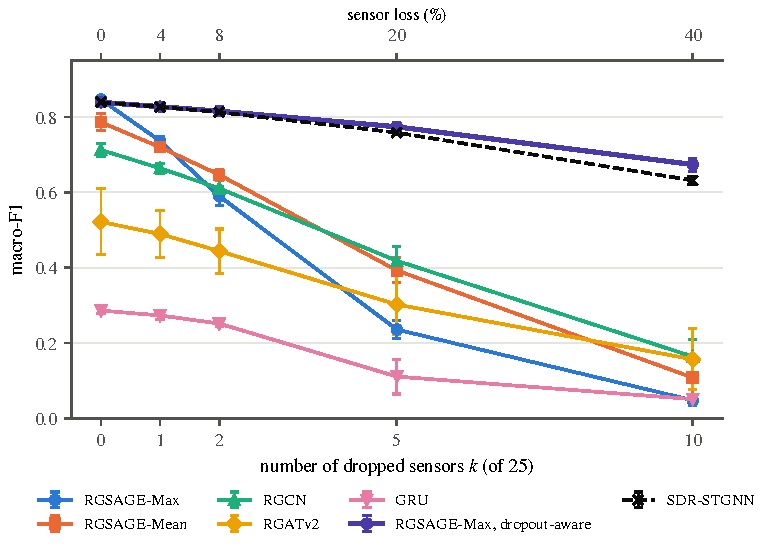
\includegraphics[width=0.78\textwidth]{fig4_1_degradation.pdf}
\caption{Degradation curves of the baselines and of the two mitigations.}
\label{fig:degradation}
\end{figure}

The inversion does not depend on the normalization by the clean score. The absolute area under the curve places RGCN (0.432) above RGSAGE-Max (0.340), and the curves cross in absolute macro-F1. The relative lead of RGATv2 is an artifact of its low clean score. Its relative area of 0.626 falls to 0.324 in absolute terms, which is the fourth of five, so the thesis does not claim RGATv2 as robust. The comparison with the trivial reference of 0.0256 shows what collapse means: at $k=10$ RGSAGE-Max reaches 0.048, only 1.9 times the score of a classifier that always answers no fault.

The split of the score into detection and localization sharpens this picture. For the standard RGSAGE-Max at $k=0$ the no-fault class has an F1 of 0.990 and the 25 fault classes have a mean F1 of 0.841. At $k=10$ the no-fault F1 is still 0.201, but the localization score has fallen to 0.041. Sensor loss destroys localization before it destroys detection.

\section{Dropout-Aware Training}

Dropout-aware training changes the picture, as Table~\ref{tab:aware} shows. For RGSAGE-Max the macro-F1 at $k=10$ rises from 0.048 to $0.674\pm0.017$, a gain of 0.626, and the retention rises from 5.7\% to 80.3\%. The relative \ac{AUDC} rises from 0.402 to 0.913. The clean score changes from $0.846\pm0.007$ to $0.839\pm0.011$, which is within one standard deviation. The gain holds for all five architectures, but the cost in clean accuracy is not the same for all of them. RGSAGE-Max loses less than 0.01 macro-F1 at $k=0$, whereas RGCN drops by 0.099 and RGSAGE-Mean by 0.113. The statement that robustness comes without a cost in clean accuracy therefore holds for the RGSAGE-Max backbone and not for the whole family. The recurrent baseline also improves, but its retention remains limited to 25\%, because it has no message passing with which to use the surviving sensors.

\begin{table}[htbp]
\caption{Effect of dropout-aware training (DA) on all architectures: macro-F1 at $k=0$ and $k=10$, relative \acs{AUDC} and retention at $k=10$ for standard (Std) and dropout-aware training.}
\label{tab:aware}
\small
\centering
\begin{tabular}{@{}lcccccccc@{}}
\toprule
 & \multicolumn{2}{c}{$k=0$} & \multicolumn{2}{c}{$k=10$} & \multicolumn{2}{c}{AUDC} & \multicolumn{2}{c}{Ret@10 (\%)} \\
\cmidrule(lr){2-3}\cmidrule(lr){4-5}\cmidrule(lr){6-7}\cmidrule(lr){8-9}
Model & Std & DA & Std & DA & Std & DA & Std & DA \\
\midrule
RGSAGE-Max & 0.846 & 0.839 & 0.048 & 0.674 & 0.402 & 0.913 & 5.7 & 80.3 \\
RGSAGE-Mean & 0.786 & 0.673 & 0.108 & 0.550 & 0.541 & 0.922 & 13.8 & 81.9 \\
RGCN & 0.712 & 0.613 & 0.164 & 0.533 & 0.608 & 0.940 & 23.2 & 87.0 \\
RGATv2 & 0.522 & 0.553 & 0.157 & 0.505 & 0.626 & 0.961 & 31.0 & 91.4 \\
GRU & 0.286 & 0.300 & 0.051 & 0.078 & 0.522 & 0.781 & 17.9 & 25.4 \\
\bottomrule
\end{tabular}
\end{table}

\section{Comparison of Remedies}

Table~\ref{tab:remedies} compares all the ways of coping with sensor loss on the RGSAGE-Max backbone under the same masks. Replacing dropped sensors by the mean of their neighbors helps little: the relative \ac{AUDC} rises from 0.402 to 0.476 and the retention at $k=10$ from 5.7\% to 11.8\%. The reconstructed values still reach a model that was never trained to distrust them. A learned graph imputer reconstructs the dropped voltages with a root-mean-square error of 0.012 to 0.017 p.u. against 0.24 to 0.30 p.u. for the neighbor mean, a reduction by a factor of 18 to 20. Its classification gain is nevertheless modest (\ac{AUDC} 0.570, retention 22.2\%), and it does not survive correction for multiple tests over the neighbor-mean fill or over zeroing. The imputer did not fully converge for two of three seeds, since its validation loss was still changing by more than the 2\% criterion at the end of 60,000 steps. A fill from the physical operator, described in Section~\ref{sec:physics}, performs better than the learned imputer (\ac{AUDC} 0.601, retention 26.6\%) but has a very large seed variance at high $k$, because a wrong best hypothesis under heavy loss produces a badly wrong fill. All three fills stay far below dropout-aware training.

\begin{table}[htbp]
\caption{Remedies on the RGSAGE-Max backbone, macro-F1 at each level $k$, relative \acs{AUDC} and retention at $k=10$, mean over three seeds. Imputation is a no-operation at $k=0$.}
\label{tab:remedies}
\small
\centering
\begin{tabular}{@{}lccccccc@{}}
\toprule
Variant & $k=0$ & $k=1$ & $k=2$ & $k=5$ & $k=10$ & AUDC & Ret@10 \\
\midrule
Standard (zeroing) & 0.846 & 0.736 & 0.590 & 0.236 & 0.048 & 0.402 & 5.7\% \\
Neighbor-mean imputation & 0.846 & 0.739 & 0.637 & 0.336 & 0.099 & 0.476 & 11.8\% \\
Learned graph imputation & 0.846 & 0.766 & 0.686 & 0.447 & 0.187 & 0.570 & 22.2\% \\
Physics-based imputation & 0.846 & 0.775 & 0.701 & 0.479 & 0.225 & 0.601 & 26.6\% \\
Dropout-aware training & 0.839 & 0.827 & 0.815 & 0.774 & 0.674 & 0.913 & 80.3\% \\
DA-wide ($k=10$ in training) & 0.833 & 0.823 & 0.812 & 0.776 & 0.704 & 0.928 & 84.5\% \\
\acs{SDR-STGNN} (gated) & 0.839 & 0.827 & 0.813 & 0.758 & 0.631 & 0.892 & 75.2\% \\
\bottomrule
\end{tabular}
\end{table}

Adding the level $k=10$ to the training grid (DA-wide) raises the macro-F1 at $k=10$ by 0.030 and lowers the clean score by 0.006. Both differences have the same sign in all three seeds, but neither survives correction ($p_{\mathrm{Holm}}=0.057$ for each), so the thesis keeps the original grid as the main method and reports the trade-off as a consistent observation. The availability-gated \ac{SDR-STGNN} matches dropout-aware training but does not exceed it. Its relative area is 0.892 against 0.913, and its curve lies below the ungated curve at every level from $k=1$ onward. At $k=0$ the gate is inactive, so the two dropout-aware variants score identically (0.839). The gate is not free: it raises the single-event latency by 18\% for no gain in robustness.

\section{Stress Tests}

\subsection{Harder Loss Patterns}

Table~\ref{tab:patterns} compares the loss patterns for RGSAGE-Max. Targeted loss is far more damaging than random loss in the regime in which the model is still usable. With one sensor removed, the standard model falls to $0.448\pm0.039$ against $0.736\pm0.013$ under random loss, a drop from the clean score that is 3.6 times larger. At $k=2$ the two policies give 0.361 and 0.590. Both differences have the same sign in all seeds but are not significant after correction ($p_{\mathrm{Holm}}=0.052$ and 0.067). From $k=5$ the two policies agree, since the model has collapsed in either case. Dropout-aware training is penalized by targeting as well (\ac{AUDC} 0.913 to 0.747, $p_{\mathrm{Holm}}=0.016$), so worst-case loss is a distinct stressor that the remedy does not absorb. The remedy still retains between 0.307 and 0.473 macro-F1 over the standard model under the same targeting ($p_{\mathrm{Holm}}\le0.012$ at every level), and for $k=5$ and $k=10$ its worst-case score exceeds the average-case score of the standard model (0.600 against 0.236 and 0.521 against 0.048, $p_{\mathrm{Holm}}=0.006$ and 0.012). At $k=1$ the two are indistinguishable ($+0.018$, $p_{\mathrm{Holm}}=0.333$).

\begin{table}[htbp]
\caption{Loss patterns on RGSAGE-Max, macro-F1 at four levels and relative \acs{AUDC}, standard (Std) and dropout-aware (DA) training.}
\label{tab:patterns}
\small
\centering
\begin{tabular}{@{}llccccc@{}}
\toprule
Pattern & Training & $k=1$ & $k=2$ & $k=5$ & $k=10$ & AUDC \\
\midrule
Random (reference) & Std & 0.736 & 0.590 & 0.236 & 0.048 & 0.402 \\
 & DA & 0.827 & 0.815 & 0.774 & 0.674 & 0.913 \\
Targeted & Std & 0.448 & 0.361 & 0.206 & 0.048 & 0.299 \\
 & DA & 0.755 & 0.695 & 0.600 & 0.521 & 0.747 \\
Persistent & Std & 0.737 & 0.592 & 0.233 & 0.047 & 0.401 \\
 & DA & 0.827 & 0.815 & 0.776 & 0.672 & 0.913 \\
Clustered & Std & 0.737 & 0.664 & 0.452 & 0.153 & 0.553 \\
 & DA & 0.827 & 0.812 & 0.762 & 0.666 & 0.904 \\
\bottomrule
\end{tabular}
\end{table}

Persistent loss, in which the dropped set is held for the whole event, changes nothing. No point of either curve moves by more than 0.003, and no difference survives correction across the twelve paired comparisons (smallest $p_{\mathrm{Holm}}=0.46$). The reason is that the decision rule is per window: the soft vote pools the 25 nodes of one window and never the 40 windows of an event, so the prediction of a window depends only on its own mask, whose distribution is the same under both schemes. This equivalence would not hold for a decision rule at the level of the event.

Clustered loss is milder than scattered loss for the standard RGSAGE-Max, with an \ac{AUDC} of 0.553 against 0.402 and a retention at $k=10$ of 18.1\% against 5.7\%. Only the difference at $k=5$ (0.452 against 0.236) survives correction ($p_{\mathrm{Holm}}=0.023$). For the dropout-aware model the two policies give nearly the same curve, with an \ac{AUDC} of 0.904 against 0.913 and no difference above 0.012 macro-F1. The gain of the remedy over the standard model remains significant at every level under clustered loss ($p_{\mathrm{Holm}}\le0.022$). The result is reported as an observation and not as an established effect, because a connected block does not drop every sensor equally often. At $k=10$ the per-node drop rate ranges from 0.18 to 0.87 against 0.40 under random loss, so the comparison does not isolate spatial correlation.

\subsection{Measurement Noise}

Noise costs real accuracy, and dropout-aware training does not protect against it (Table~\ref{tab:noise}). For the standard RGSAGE-Max at $k=0$ the macro-F1 falls from 0.846 to 0.786, 0.579 and 0.345 at noise levels of 0.0005, 0.002 and 0.01 p.u. The largest level is the one percent limit of the synchrophasor standard. Dropout-aware training is not better at any noise level at $k=0$, and the differences from the standard model range from $-0.008$ to $-0.034$, with confidence intervals that include zero. The explanation follows from the mechanism of the remedy. Noise leaves the availability mask at one, so the learned response to a node that is dark has nothing to react to. The advantage of the remedy against sensor loss survives noise in attenuated form: at $k=10$ the gain over the standard model is $+0.627$ without noise and $+0.579$, $+0.428$ and $+0.209$ with increasing noise. Noise and sensor loss compound below the trivial reference. The standard model at $k=10$ and the largest noise level scores 0.018, below the 0.0256 of a classifier that always answers no fault.

\begin{table}[htbp]
\caption{RGSAGE-Max under measurement noise and sensor loss, macro-F1 for standard (Std) and dropout-aware (DA) training.}
\label{tab:noise}
\small
\centering
\begin{tabular}{@{}lcccccccc@{}}
\toprule
 & \multicolumn{4}{c}{$k=0$} & \multicolumn{4}{c}{$k=10$} \\
\cmidrule(lr){2-5}\cmidrule(lr){6-9}
$\sigma$ (p.u.) & 0 & 0.0005 & 0.002 & 0.01 & 0 & 0.0005 & 0.002 & 0.01 \\
\midrule
Std & 0.846 & 0.786 & 0.579 & 0.345 & 0.048 & 0.040 & 0.032 & 0.018 \\
DA & 0.839 & 0.752 & 0.555 & 0.316 & 0.675 & 0.619 & 0.460 & 0.227 \\
\bottomrule
\end{tabular}
\end{table}

\subsection{Unseen Fault Scenarios}

The event-level split leaves every scenario in all three splits. On the split that holds out whole scenarios, accuracy is much lower, which is the largest limit on the generalization of the reported scores. The standard RGSAGE-Max reaches $0.490\pm0.057$ at $k=0$, against 0.846 on the event-level split, and the dropout-aware model reaches $0.384\pm0.030$. Under sensor loss the standard model falls to 0.066 at $k=10$, and the dropout-aware model keeps 0.265. The models therefore generalize to unseen load conditions of known fault configurations far better than to unseen configurations. This split was evaluated only for RGSAGE-Max, without statistical tests, so these numbers describe the size of the effect and not a tested ranking.

\subsection{Classical Baselines and the Detection--Localization Split}

A logistic regression on 375 summary features reaches a macro-F1 of 0.713 at $k=0$ and a random forest reaches 0.633, both trained on 8\% of the training windows and without any graph. The margin of RGSAGE-Max over the linear model is 0.133 and not the 0.560 that the recurrent baseline suggests. Under sensor loss the random forest is the most robust of the untreated models: it keeps 35.9\% of its clean score at $k=10$, with an absolute area of 0.470, above the 0.432 of RGCN. The linear model collapses to 0.039. The dropout-aware RGSAGE-Max, with a retention of 80.3\% and an absolute area of 0.766, is more robust than any of them.

\section{Statistical Significance}

Paired two-sided $t$-tests on the mitigation claims, over the three training seeds and with Holm correction across the seven tests of the family, support the mitigation claims ($\mathrm{df}=2$). Dropout-aware training improves the macro-F1 at $k=10$ by 0.626, the retention by 74.6 percentage points and the area by 0.511, and all three survive correction ($p_{\mathrm{Holm}}=0.004$). It also exceeds neighbor-mean imputation by 0.574 ($p_{\mathrm{Holm}}=0.010$) and the learned imputer by 0.486 ($p_{\mathrm{Holm}}=0.037$). The area gain is significant for each of the five architectures ($p_{\mathrm{Holm}}\le0.027$), and the gain is significant at every level $k\ge1$ ($p_{\mathrm{Holm}}\le0.042$). The two null claims of this thesis also test as null. The clean-accuracy cost of $-0.008$ has an interval that includes zero ($p_{\mathrm{Holm}}=0.196$), and the advantage of dropout-aware training over \ac{SDR-STGNN} in the area is also not significant ($p_{\mathrm{Holm}}=0.196$), which is the statistical form of the statement that the gate matches but does not exceed it.

Two orderings of the baselines are not significant at three seeds. The clean ranking of the top pair, RGSAGE-Max over RGSAGE-Mean, has $p_{\mathrm{Holm}}=0.085$ and no adjacent pair survives. The accuracy--robustness inversion, in which RGCN exceeds RGSAGE-Max at $k=10$ in every seed by a factor of 2.4 to 6.7 ($+0.116$), has $p_{\mathrm{Holm}}=0.429$ because the size of the gap varies from seed to seed. A bootstrap over the 6,175 test events gives an interval for the top pair about five times narrower than the seed-level interval, so the number of training seeds limits these orderings, and they are reported as consistent observations. The spread between mask realizations within a seed (0.0002 to 0.0046 macro-F1) is small against the spread between seeds (0.008 to 0.061).

\section{Computational Cost}

Dropout-aware training changes only the data. The standard and the dropout-aware RGSAGE-Max have the same 95,258 parameters and the same single-event latency (0.639 against 0.640 ms), and both process 6,038 windows per second. The only extra cost is 2.7\% in training time per epoch. \ac{SDR-STGNN} adds no parameters but raises the latency by 18\% (0.755 against 0.639 ms) for no robustness gain. A training run takes between 4.7 and 12.3 hours on the NVIDIA T1000 for the five architectures, 6.7 hours for standard and 6.9 hours for dropout-aware RGSAGE-Max.

\section{The Physical Operator}
\label{sec:opresults}

\subsection{Fidelity of the Signature Table}

The checks of Section~\ref{sec:physics} support the table. The median bias of the table against the corpus at the true hypothesis is $1.3\times10^{-3}$ p.u. Profiling the load and the type at the true location recovers the load multiplier within one grid step for 97.3\% of the 28,875 training events and the fault type for 90.9\%. The residual floor, rescaled by one global constant chosen on the training split, gives a median squared residual per channel of 1.00 at the true class, and halving the resistance grid changes the localization macro-F1 on the 25 fault classes by $-0.0013$, within noise. The bias check is a construction check, because the table is the generator of the corpus run again. A build with a standing circuit disagreed with the corpus by more than $10^{-3}$ p.u. on 43.3\% of 1,000 tested events, against 1.8\% when the circuit was compiled again for every solution.


\subsection{Identifiability}

The separability of Eq.~\eqref{eq:sep} shows that 25 magnitude-only sensors carry enough information to separate almost every pair of fault locations. Of the 325 pairs among the 26 classes, 1.5\% are indistinguishable at the floor of the operator for $k=0$, 2 and 5, and 1.8\% for $k=10$. The most confusable pair is the same at every level, and its separability falls from 0.0074 to 0.0047. The limit is a property of high resistance and not of the number of sensors: at 0.1 and 1~$\Omega$ no pair is indistinguishable at any level, and at 10~$\Omega$ the fraction is 0.6\% at $k=0$ and 2 and 0.9\% at $k=5$ and 10. Figure~\ref{fig:ident} shows the separability maps. The table agrees with the empirical confusability of the raw observations: a nearest-neighbor classifier on the 55 instrumented channels reaches an accuracy of 88.9\%, and the rank correlation between the separability of a pair and its empirical confusion is $-0.655$ with $p=4\times10^{-38}$ over 300 location pairs. No pair that the table calls confusable is separable in the corpus.

\begin{figure}[htbp]
\centering
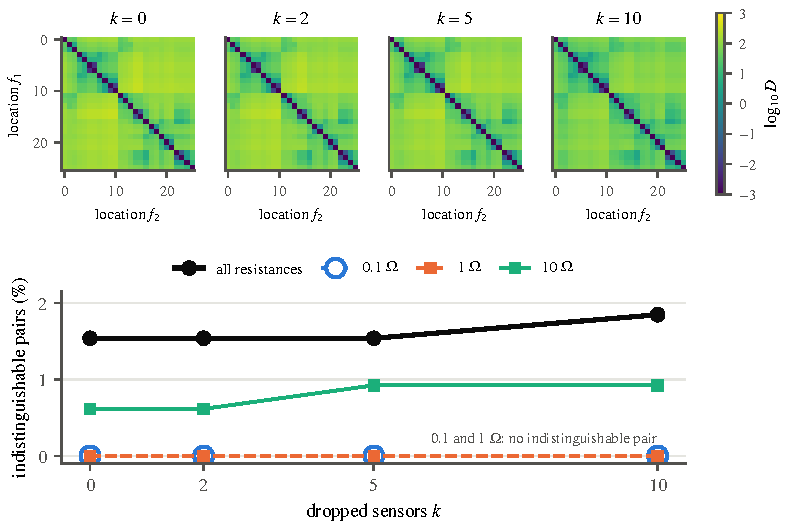
\includegraphics[width=0.9\textwidth]{fig4_3_identifiability.pdf}
\caption{Identifiability of the fault location from 25 magnitude-only sensors.}
\label{fig:ident}
\end{figure}

\subsection{Physics-Only Baselines}

The training-free methods are ordered on the validation split with the same 26-class window-level macro-F1 as the networks. A rank-one sag template without profiling scores 0.162 at every level and is almost uninformative on its own. Matching the nearest signature at the nominal load, without profiling, scores 0.649 at $k=0$ and 0.601 at $k=10$. Profiling the type, the resistance and the load (\ac{PSM}) adds 0.123 and scores 0.772 at $k=0$. The score of \ac{PSM} is nearly flat under sensor loss, since the residual simply drops the lost channels from its sum, and it falls only to 0.749 at $k=10$ (absolute area 0.762). In distribution, the learned model is better: the dropout-aware RGSAGE-Max reaches 0.855 on the validation split at $k=0$ for the same seed. The physical operator therefore does not win on its own ground, and its score on clean data is a check of fidelity and not a competitor of the learned model, since the table and the corpus come from the same simulator. Its value lies in the perturbed conditions, as the next subsection shows.


\subsection{Inference-Time Fusion}

Combining the residual with an existing dropout-aware checkpoint at inference, as in Eq.~\eqref{eq:fusion}, raises the score in every condition tested. The gain is small on clean data (0.858 to 0.897, $+0.039$) and large where the network has the least to work with: $+0.166$ at $k=10$ (0.695 to 0.860), $+0.086$ for faults of 10~$\Omega$ (0.667 to 0.753), and up to $+0.213$ at the noise level of 0.01 p.u. (0.325 to 0.538). Noise levels of 0.0005 and 0.002 p.u. give $+0.037$ and $+0.153$. The level of 0.01 p.u. is the condition against which dropout-aware training has no effect. The weight $\beta$ that the validation selects is 0.1 except at the two highest noise levels, where it is 16 and 2. These are preliminary results: they use one seed, a subsample of 30,000 validation windows, and a weight chosen on the same data on which it is scored, and the fusion was applied to a checkpoint that was never trained to expect it.


Computing the residual online takes 44.7 ms for a batch of 32 on the T1000, nine times more than the budget set for it. For the offline evaluation the residual of the whole corpus was therefore computed once and stored for all dropout levels and mask realizations. The stored values agree with the online computation to a relative error of $1.6\times10^{-5}$ and select the same hypothesis in all cases.

\subsection{Screening of Three First-Order Physics Grafts}

Before the operator was built, three ways of adding first-order physical knowledge to the RGSAGE-Max backbone were screened, each with at most one extra parameter: messages scaled by the impedance of the edge between two sensors, a bias from a shared-path sensitivity on the logits, and a loss that penalized the mismatch of the sag pattern. At seed 42 and with 15 epochs, none improved on the backbone, whose validation score at epoch 15 was 0.816, against 0.807, 0.811 and 0.811 for the three variants. The weight of the first prior was driven to zero, and the sign of the second was reversed. The third, run at the full recipe and three seeds, matches the baseline in clean accuracy ($0.847\pm0.018$ against $0.846\pm0.007$) and with dropout-aware training ($0.837$ against $0.839$), makes training less stable, and lost its apparent advantage against noise ($-0.032$ at the largest noise level). The physics available in voltage magnitudes alone is weak when it is injected in these ways, which motivated the stronger operator of the preceding sections.


\section{PC-STGNN}
\label{sec:pcresults}

\subsection{Verification}

The checks of Section~\ref{sec:pcstgnn} passed. With $\lambda_1=\lambda_2=\beta=0$ the model reproduced all 30 epochs of the dropout-aware backbone exactly, with identical training loss, validation scores and best validation score (0.8555). With $\gamma=0$ the new objective gave the same loss and identical gradients for all 17 parameter tensors on a fixed batch. The finite-difference audit passed on all three batches: both physical terms sent a non-zero gradient to the network weights, $\beta$ received a gradient, the signature table received none, and the leave-$k$-out term vanished without undefined values when no sensor was dropped.

\subsection{Noise Augmentation for Noise Robustness and the Auxiliary Loss Against Collapse}

Trained without noise, all six tuning arms converged to a degenerate solution. On the 248,000 validation windows at $k=0$, the network branch alone predicted no fault for 99.9 to 100\% of the windows and scored 0.0256, the trivial reference, while the fused prediction agreed with \ac{PSM} on between 87.7\% and 98.0\% of the fault windows. The model had become physics matching with a learned no-fault bias, as the design analysis had predicted: when the residual at the true class is exactly zero, trusting it completely is the easiest solution.

Noise augmentation reduced the problem but did not remove it. The network branch predicted no fault for about 55\% of the windows, close to the true 50\%, but its macro-F1 stayed at 0.078 without the physical loss and 0.061 with it, below the criterion of 0.10. The auxiliary loss on the network-only logits resolved it. After five epochs with $\gamma=1$, the network branch alone reached a macro-F1 of 0.571, 7.3 times the value without the auxiliary term, and the fused score stayed at 0.879. The auxiliary term is therefore fixed at $\gamma=1$ and is part of the model. A model trained for 30 epochs at seed 42 with $\gamma=1$ and without noise augmentation did not collapse. Without noise at test time, its network branch alone scored 0.828 at $k=0$, against 0.807 for the noise-trained model at the same seed, and its fused score was lower than that of the noise-trained model by 0.008 to 0.014 at the five sensor-loss levels. With noise added at test time, it scored lower in all 15 conditions, by 0.075 to 0.259, and at noise levels of 0.002 p.u. and above its fused macro-F1 was below that of \ac{PSM} alone in all 10 conditions. This is a single seed and no significance is claimed. It gives no evidence that noise augmentation is needed to prevent the collapse when $\gamma=1$, but it shows that noise augmentation is needed for robustness to noise.

\subsection{Selection of the Loss Weights}

The final tuning compared five arms, all with noise and the auxiliary loss, at one seed and 15 epochs, and all passed the collapse guard. The loss $\lambda_1$ hurts monotonically: the validation score averaged over the sensor-loss levels falls from 0.878 at $\lambda_1=0$ to 0.852 at 0.0333 and 0.818 at 0.1, and the loss shows up in the no-fault windows, where the fused accuracy falls from 100.0\% to 74.2\% because a larger $\beta$ lets the physics override correct no-fault decisions. The expected residual on the available sensors therefore does not contribute. The held-out term with $\lambda_2=0.1$ is neutral to slightly positive. The best averaged score is 0.880, which selects $\lambda_1=0$ and $\lambda_2=0.1$, but the margin of 0.002 over $\lambda_1=\lambda_2=0$ is not a tested difference. Even at the end of this tuning, the fused prediction on fault windows agrees with \ac{PSM} for 91.5 to 94.7\% of the windows, so at clean $k=0$ the localization is still largely physical. The behavior under noise and sensor loss is the subject of the next subsection.


\subsection{Comparison With the Noise-Augmented Reference}

The comparison that decides whether the learned fusion helps is between \ac{PC-STGNN} and the noise-augmented reference model. Both are trained for 30 epochs at seeds 42, 43 and 44 and evaluated on the validation split at every combination of the noise levels and the sensor-loss levels of Section~\ref{sec:pcstgnn}. The two models of one seed form a pair, and a difference is sign-consistent when it has the same sign in all three pairs. The decision rule was fixed before training: the fused model must score higher in all three seeds at every condition that can be evaluated before the test on unseen fault resistances, namely faults of 10~$\Omega$, sensor loss and measurement noise. Sign consistency is the primary criterion and does not depend on a significance test. A Holm correction is reported in addition for the seven conditions with sensor loss ($k\in\{1,2,5,10\}$ without noise and $k=10$ at each noise level). This family was chosen after the results were seen, so it describes where the result is strongest and is not part of the decision. The test on unseen resistances is made later, on a separate set, and is not part of this comparison.

Table~\ref{tab:gate4} gives the macro-F1 of every seed. \ac{PC-STGNN} scores higher than the reference in all 60 pairs of seed and condition, and the smallest single difference is 0.008, so the primary criterion is met at every evaluated condition. For faults of 10~$\Omega$ without noise or sensor loss, \ac{PC-STGNN} also scores higher in all three seeds (0.733, 0.753 and 0.736, against 0.635, 0.632 and 0.657). The mean difference grows with the number of lost sensors, from 0.059 at $k=0$ to 0.201 at $k=10$ without noise, and it decreases as the noise rises, to 0.025 at $k=0$ and 0.101 at $k=10$ at 0.01 p.u. In the seven-condition family, all differences are significant after the Holm correction ($p_{\mathrm{Holm}}\le0.020$). With three seeds, the significance depends on the size of the family: over all twenty conditions, only the two largest differences, at $k=10$ without noise and at 0.0005 p.u., remain significant ($p_{\mathrm{Holm}}=0.025$), and at $k=0$ and 0.01 p.u. the difference is not significant even before the correction ($p=0.14$).

The reference was still improving at the end of training. Its best validation epochs were 30, 29 and 27, and its mean validation score over epochs 26 to 30 was 0.010 to 0.016 higher than over epochs 21 to 25. The best epochs of \ac{PC-STGNN} were 19, 29 and 17, and its score changed by less than 0.005 between the same two periods. The reference is therefore compared before it reached its final level, and the margins can decrease with longer training.

\begin{table}[htbp]
\caption{Comparison of \acs{PC-STGNN} with the noise-augmented reference, validation macro-F1 per training seed. The difference is the mean over the three seed pairs. $p_{\mathrm{Holm}}$ is given for the seven conditions of the decision family; the other conditions are descriptive.}
\label{tab:gate4}
\footnotesize
\centering
\begin{tabular}{@{}rlcccccccc@{}}
\toprule
 & & \multicolumn{3}{c}{Reference} & \multicolumn{3}{c}{\acs{PC-STGNN}} & & \\
\cmidrule(lr){3-5}\cmidrule(lr){6-8}
$k$ & Noise (p.u.) & 42 & 43 & 44 & 42 & 43 & 44 & Difference & $p_{\mathrm{Holm}}$ \\
\midrule
0 & 0 & 0.846 & 0.831 & 0.841 & 0.895 & 0.902 & 0.897 & $+0.059$ & -- \\
 & 0.0005 & 0.846 & 0.830 & 0.838 & 0.897 & 0.899 & 0.896 & $+0.059$ & -- \\
 & 0.002 & 0.829 & 0.810 & 0.819 & 0.868 & 0.874 & 0.872 & $+0.052$ & -- \\
 & 0.01 & 0.736 & 0.714 & 0.721 & 0.744 & 0.758 & 0.743 & $+0.025$ & -- \\
\addlinespace
1 & 0 & 0.833 & 0.817 & 0.826 & 0.891 & 0.897 & 0.893 & $+0.068$ & 0.020 \\
 & 0.0005 & 0.833 & 0.817 & 0.824 & 0.892 & 0.894 & 0.891 & $+0.068$ & -- \\
 & 0.002 & 0.818 & 0.798 & 0.806 & 0.861 & 0.869 & 0.866 & $+0.058$ & -- \\
 & 0.01 & 0.728 & 0.705 & 0.711 & 0.738 & 0.752 & 0.737 & $+0.028$ & -- \\
\addlinespace
2 & 0 & 0.820 & 0.804 & 0.811 & 0.887 & 0.893 & 0.889 & $+0.078$ & 0.020 \\
 & 0.0005 & 0.820 & 0.803 & 0.809 & 0.888 & 0.890 & 0.887 & $+0.077$ & -- \\
 & 0.002 & 0.804 & 0.786 & 0.792 & 0.855 & 0.863 & 0.860 & $+0.065$ & -- \\
 & 0.01 & 0.719 & 0.696 & 0.701 & 0.732 & 0.746 & 0.732 & $+0.031$ & -- \\
\addlinespace
5 & 0 & 0.776 & 0.757 & 0.761 & 0.875 & 0.877 & 0.878 & $+0.112$ & 0.017 \\
 & 0.0005 & 0.776 & 0.757 & 0.759 & 0.876 & 0.877 & 0.876 & $+0.112$ & -- \\
 & 0.002 & 0.762 & 0.742 & 0.746 & 0.837 & 0.846 & 0.842 & $+0.092$ & -- \\
 & 0.01 & 0.686 & 0.662 & 0.663 & 0.713 & 0.727 & 0.714 & $+0.048$ & -- \\
\addlinespace
10 & 0 & 0.669 & 0.650 & 0.647 & 0.856 & 0.856 & 0.858 & $+0.201$ & 0.009 \\
 & 0.0005 & 0.669 & 0.650 & 0.647 & 0.853 & 0.854 & 0.854 & $+0.199$ & 0.009 \\
 & 0.002 & 0.658 & 0.638 & 0.636 & 0.802 & 0.811 & 0.811 & $+0.164$ & 0.017 \\
 & 0.01 & 0.595 & 0.572 & 0.568 & 0.673 & 0.690 & 0.674 & $+0.101$ & 0.020 \\
\bottomrule
\end{tabular}
\end{table}

Table~\ref{tab:decomp} separates the fused output of \ac{PC-STGNN} into the soft vote of the network branch alone and the \ac{PSM} prediction from the residual alone. The fused score is higher than both sources in every condition, by 0.038 to 0.132. The two sources fail under different perturbations. Sensor loss lowers the network branch from 0.812 at $k=0$ to 0.615 at $k=10$ without noise, but it lowers \ac{PSM} only from 0.772 to 0.750. Noise lowers \ac{PSM} from 0.772 to 0.496 at $k=0$, and the network branch only from 0.812 to 0.710. The fused class follows the source that holds up: at $k=0$, its agreement with \ac{PSM} falls from 71.3\% without noise to 34.4\% at 0.01 p.u., and without noise its agreement with the network branch falls from 92.1\% at $k=0$ to 82.2\% at $k=10$. In every condition the fused class agrees with the network branch more often than with \ac{PSM}. The agreement is counted over all windows, including the no-fault windows, in which \ac{PSM} is weak, so it does not measure the share of physical evidence in the fault decisions alone.

\begin{table}[htbp]
\caption{Sources of the fused prediction of \acs{PC-STGNN} at $k=0$ and $k=10$, validation split, mean over three seeds. The columns give the macro-F1 of the fused output, of the network branch alone and of \acs{PSM}, and the percentage of all windows in which the fused class equals the class of each source.}
\label{tab:decomp}
\footnotesize
\centering
\begin{tabular}{@{}rlccccc@{}}
\toprule
 & & \multicolumn{3}{c}{Macro-F1} & \multicolumn{2}{c}{Agreement of the fused class (\%)} \\
\cmidrule(lr){3-5}\cmidrule(lr){6-7}
$k$ & Noise (p.u.) & Fused & Network only & \acs{PSM} & With network & With \acs{PSM} \\
\midrule
0 & 0 & 0.898 & 0.812 & 0.772 & 92.1 & 71.3 \\
 & 0.0005 & 0.897 & 0.811 & 0.770 & 92.6 & 70.5 \\
 & 0.002 & 0.871 & 0.796 & 0.746 & 94.7 & 65.2 \\
 & 0.01 & 0.748 & 0.710 & 0.496 & 97.4 & 34.4 \\
\addlinespace

10 & 0 & 0.857 & 0.615 & 0.750 & 82.2 & 70.2 \\
 & 0.0005 & 0.854 & 0.614 & 0.747 & 82.8 & 69.0 \\
 & 0.002 & 0.808 & 0.606 & 0.704 & 86.2 & 60.0 \\
 & 0.01 & 0.679 & 0.547 & 0.457 & 91.9 & 30.2 \\
\bottomrule
\end{tabular}
\end{table}

The comparison does not identify which element of \ac{PC-STGNN} produces the gain. The model differs from the reference in the fused residual, the held-out term with $\lambda_2=0.1$ and the auxiliary loss with $\gamma=1$. The expected residual is not among them, because $\lambda_1=0$. The data show where the gain is realized. The network branch of \ac{PC-STGNN} alone scores below the reference in 45 of the 60 pairs, with a mean deficit per condition between 0.014 and 0.041, and only the fused output is better than the reference. The gain therefore arises in the fusion step and not through a stronger network branch. One single-seed ablation was completed: a model trained for 30 epochs with the same noise augmentation and the held-out term, but without the auxiliary loss ($\gamma=0$). At its selected checkpoint, epoch 8, the network branch alone localized poorly: its macro-F1 was between 0.055 and 0.080 in all twenty conditions (0.079 at $k=0$ without noise), against 0.55 to 0.81 for the model with $\gamma=1$ at the same seed, a deficit of 0.49 to 0.73. At epoch 30 the network-only score had risen to 0.21 at $k=0$ without noise, which is still far below. The fused macro-F1 was lower than that of the $\gamma=1$ model in 19 of the 20 conditions, by 0.009 on average (the largest difference is 0.018 and one condition is higher by 0.001), and at $k=0$ without noise the fused class agreed with the network branch for 56\% of the windows instead of 92\%. With one seed no significance is claimed, and the result supports only a statement about the network branch: without the auxiliary loss the network branch alone does not localize faults, even with noise augmentation. The other ablations that separate the three elements, and the test of whether the gain needs the correct assignment of signatures to locations, were not completed and are left for future work.

\section{Discussion}

Four findings stand out. First, clean accuracy is an unreliable guide to robustness. The model that is best with all sensors is the most fragile when they fail, in absolute as well as relative terms, although the ordering of the middle models is indicative only at three seeds. The max aggregation forwards the largest activation of a neighborhood, so one corrupted message can dominate a live node, whereas the normalized sum and the mean average it away.

Second, the remedy works because it changes what the mask means. In the clean corpus the mask channels are static: they identify the phase instrumentation of a unit and never change, so a standard model reads the mask as a fixed fingerprint of the node and not as a live signal. A dropped sensor shows the all-zero pattern, which that node never shows in training, so the model reads the zero voltages as a valid near-zero measurement. Dropout-aware training makes the mask vary within the history of a node, so the all-zero pattern acquires the meaning that the neighbor is dark. This account fits three observations. An explicit gate is redundant, because the model has learned what the gate hard-codes. Plausible numbers do not replace the training signal, because the deficit is misplaced trust and not a lack of values. And the gain is smallest for the recurrent baseline, which has no path for information to route around a dark node. The same account explains why noise defeats the remedy: noise leaves the mask at one.

Third, the conclusions have limits. Scores on the event-level split fall by about 0.36 on unseen scenarios for the standard model, worst-case loss and noise are stressors that the remedy does not absorb, and the data are quasi-static magnitudes from one simulated feeder.

Fourth, the physical operator is informative but does not replace the learned model. Fusion at inference helps most under noise and heavy sensor loss in the preliminary test, whereas injection through the loss was neutral or harmful, and in the tuning at one seed the network branch collapsed without the auxiliary loss. Trained at three seeds, the fusion scores higher than the noise-augmented reference in every seed and condition, most under sensor loss (Table~\ref{tab:gate4}). The network branch and the physical prediction fail under different perturbations, and the fused output is better than each of them (Table~\ref{tab:decomp}). The comparison does not separate which element of the model produces the gain.

\section{Summary}

The most accurate model is the most fragile, and dropout-aware training restores 80.3\% of the clean score at 40\% sensor loss at no inference cost. Neither a gate nor imputation matches it. A fixed physical operator is informative and, fused into the network with one learned parameter, raised the validation macro-F1 over a noise-augmented reference in every seed and condition tested, most under heavy sensor loss.

\chapter{Conclusion and Future Enhancements}
\label{chap:conclusion}

\section{Summary of the Work}

The thesis studied what happens to a learned fault localizer on a sparsely instrumented feeder when sensors fail or are noisy after deployment. It adopted the framework of \citet{karabulut2026} on the IEEE 123-bus feeder, regenerated a corpus of 1.65 million windows and benchmarked five architectures at three seeds. It measured their degradation under sensor loss, developed dropout-aware training as a remedy and compared it with an availability-gated architecture and with three kinds of imputation. It then tested the conclusions under harder conditions, built a fixed physical operator from simulated fault signatures, and designed a physics-consistent model.

\section{Conclusions}

The conclusions follow the research questions of Section~\ref{sec:rq}.

\textbf{RQ1: degradation and its relation to accuracy.} Localization degrades sharply with sensor loss. The most accurate baseline, RGSAGE-Max, falls from 0.846 to 0.048 when 10 of 25 sensors are lost and keeps only 5.7\% of its clean score. Clean accuracy is an unreliable guide to robustness: the accuracy ranking of the five baselines is essentially reversed by the robustness ranking, in absolute as well as relative terms. Sensor loss destroys localization before detection.

\textbf{RQ2: remedies.} Dropout-aware training raises the macro-F1 of RGSAGE-Max at 40\% sensor loss from 0.048 to 0.674 and the retention from 5.7\% to 80.3\% ($p_{\mathrm{Holm}}=0.004$), at no cost in parameters or latency and with 2.7\% more training time per epoch. It improves the area under the retention curve for all five architectures, although for RGCN and RGSAGE-Mean it costs about 0.1 macro-F1 under full observability. The availability-gated model matches the remedy but does not exceed it, and it adds 18\% to the latency. Neighbor-mean, learned and physics-based imputation recover little, because a model that was never trained to distrust the filled values still trusts them.

\textbf{RQ3: harder conditions.} The advantage of the remedy persists under persistent and clustered loss, but two conditions limit it. Targeted loss of the sensors nearest the fault is a distinct stressor that the remedy does not absorb, since its area falls from 0.913 to 0.747, although the remedy still outperforms the standard model under the same targeting. Measurement noise defeats the remedy completely at full observability, because noise leaves the availability mask unchanged and the learned response to a dark node has nothing to react to. On the scenario-held-out split the standard model falls from 0.846 to 0.490, so the reported accuracy holds for unseen loads and not for unseen fault configurations.

\textbf{RQ4: information content of the sensors.} Twenty-five magnitude-only sensors carry enough information to separate almost every pair of fault locations: 1.5\% of the pairs are indistinguishable for $k=0$ to 5 and 1.8\% for $k=10$, and the limit lies at high resistance and not in the number of sensors. The physical operator does not beat the learned model on its own ground, since training-free matching reaches 0.772 against 0.855 for the learned model on the validation split. It is nearly insensitive to sensor loss and, applied at inference to a trained checkpoint, improved the score in every condition tested in a preliminary test, most strongly under noise and heavy sensor loss.

\textbf{RQ5: fusion in the network.} The fusion adds one parameter, reduces exactly to the backbone when switched off, and sends gradient to the network weights and not to the fixed table. Its design needed noise augmentation and an auxiliary loss on the network-only logits: in the tuning at one seed, the network learned to defer entirely to the physics without them. A single-seed run with the auxiliary loss and without noise augmentation did not defer to the physics, so there is no evidence that noise augmentation is needed for this purpose, although it is needed for robustness to noise. A single-seed run of 30 epochs without the auxiliary loss, but with noise augmentation, confirmed the second element for the network branch: its network-only macro-F1 was 0.055 to 0.080 against 0.55 to 0.81 with the auxiliary loss, while its fused macro-F1 was only 0.009 lower on average. Trained for 30 epochs at three seeds, the fused model scores higher than a reference with the same noise augmentation and no physics in every seed at all twenty combinations of noise and sensor loss (Table~\ref{tab:gate4}). The largest gain is $+0.201$ macro-F1 at $k=10$ without noise ($p_{\mathrm{Holm}}=0.009$). The comparisons under sensor loss are significant in a seven-condition family chosen after the results were seen, and the gain decreases as the noise rises and is not significant at $k=0$ with 0.01 p.u. It arises in the fusion step: the network branch alone scores below the reference in 45 of the 60 pairs, and the fused output is better than both the network branch and \ac{PSM} in every condition. The reference was still improving at its last epoch, so the margins can decrease with longer training. The comparison does not show which element of the model produces the gain, or whether the gain requires the correct physical signatures. The other ablations that would show it were not completed.

\section{Limitations}

The limitations are those of the scope in Section~\ref{sec:scope}. All data come from simulation of one feeder with a fixed sensor placement and quasi-static \ac{RMS} magnitudes, so field performance and transient content are not tested. The statistics rest on three seeds, so several orderings are only observations. The clustered comparison does not isolate spatial correlation, because a connected block drops some sensors much more often than others. The signature table comes from the simulator of the corpus, so clean-data comparisons favor the physical operator. The scenario-held-out split covers RGSAGE-Max only, and the depth of four layers was selected on it and applied to every architecture.

\section{Future Enhancements}

Several extensions follow from the work. The physics-consistent model needs ablations that test whether its gain comes from the physics: a model that keeps only the held-out term, a model without the auxiliary loss, a shuffled assignment of signatures to locations, and a learned decoder of matched size. It is also to be evaluated on resistances outside the training values, with a test set that was generated and sealed in advance, and under a perturbed signature table, to measure its tolerance to an imperfect feeder model. A sensor that keeps reporting wrong values can be studied with a per-sensor trust score derived from the residual. Other directions are the validation on additional feeders such as the IEEE 34-bus system and on reconfigured topologies, the use of voltage phase angles, joint training of an imputer and a classifier, equal drop rates in the clustered comparison, more seeds to test the observed orderings, and field \ac{UPMU} data.
%------------------------------------------------------------------------------------------------%

%%%%%%%%%%%%%%%%%%%%%%%%%%%%%%%%%%%%%%%%%%%%%%%%%%%%%%%%%%%%
% Bibliography.
\begin{singlespace}
  \bibliography{thesis_refer} %Enter your .bib file name here
\end{singlespace}
\addcontentsline{toc}{chapter}{REFERENCES}
%%%%%%%%%%%%%%%%%%%%%%%%%%%%%%%%%%%%%%%%%%%%%%%%%%%%%%%%%%%%
  \end{document}
